\documentclass[landscape,a0paper,fontscale=0.292]{baposter}

\usepackage[vlined]{algorithm2e}
\usepackage{times}
\usepackage{calc}
\usepackage{url}
\usepackage{graphicx}
\usepackage{amsmath}
\usepackage{amssymb}
\usepackage{relsize}
\usepackage{multirow}
\usepackage{booktabs}

\usepackage{graphicx}
\usepackage{multicol}
\usepackage[T1]{fontenc}
\usepackage{ae}

\graphicspath{{images/}}

 %%%%%%%%%%%%%%%%%%%%%%%%%%%%%%%%%%%%%%%%%%%%%%%%%%%%%%%%%%%%%%%%%%%%%%%%%%%%%%%%
 %%%% Some math symbols used in the text
 %%%%%%%%%%%%%%%%%%%%%%%%%%%%%%%%%%%%%%%%%%%%%%%%%%%%%%%%%%%%%%%%%%%%%%%%%%%%%%%%
 % Format 
 \newcommand{\RotUP}[1]{\begin{sideways}#1\end{sideways}}


 %%%%%%%%%%%%%%%%%%%%%%%%%%%%%%%%%%%%%%%%%%%%%%%%%%%%%%%%%%%%%%%%%%%%%%%%%%%%%%%%
 % Multicol Settings
 %%%%%%%%%%%%%%%%%%%%%%%%%%%%%%%%%%%%%%%%%%%%%%%%%%%%%%%%%%%%%%%%%%%%%%%%%%%%%%%%
 \setlength{\columnsep}{0.7em}
 \setlength{\columnseprule}{0mm}


 %%%%%%%%%%%%%%%%%%%%%%%%%%%%%%%%%%%%%%%%%%%%%%%%%%%%%%%%%%%%%%%%%%%%%%%%%%%%%%%%
 % Save space in lists. Use this after the opening of the list
 %%%%%%%%%%%%%%%%%%%%%%%%%%%%%%%%%%%%%%%%%%%%%%%%%%%%%%%%%%%%%%%%%%%%%%%%%%%%%%%%
 \newcommand{\compresslist}{%
 \setlength{\itemsep}{1pt}%
 \setlength{\parskip}{0pt}%
 \setlength{\parsep}{0pt}%
 }


 %%%%%%%%%%%%%%%%%%%%%%%%%%%%%%%%%%%%%%%%%%%%%%%%%%%%%%%%%%%%%%%%%%%%%%%%%%%%%%
 % Formating
 \newcommand{\Matrix}[1]{\begin{bmatrix} #1 \end{bmatrix}}
 \newcommand{\Vector}[1]{\begin{pmatrix} #1 \end{pmatrix}}

 \newcommand*{\norm}[1]{\mathopen\| #1 \mathclose\|}% use instead of $\|x\|$
 \newcommand*{\abs}[1]{\mathopen| #1 \mathclose|}% use instead of $\|x\|$
 \newcommand*{\normLR}[1]{\left\| #1 \right\|}% use instead of $\|x\|$

 \newcommand*{\SET}[1]  {\ensuremath{\mathcal{#1}}}
 \newcommand*{\FUN}[1]  {\ensuremath{\mathcal{#1}}}
 \newcommand*{\MAT}[1]  {\ensuremath{\boldsymbol{#1}}}
 \newcommand*{\VEC}[1]  {\ensuremath{\boldsymbol{#1}}}
 \newcommand*{\CONST}[1]{\ensuremath{\mathit{#1}}}

 \DeclareMathOperator*{\argmax}{arg\,max}
 \DeclareMathOperator*{\diag}{diag}
 \DeclareMathOperator*{\argmin}{arg\,min}
 \DeclareMathOperator*{\vectorize}{vec}
 \DeclareMathOperator*{\reshape}{reshape}

 %-----------------------------------------------------------------------------
 % Differentiation
 \newcommand*{\Nabla}[1]{\nabla_{\!#1}}

 \renewcommand*{\d}{\mathrm{d}}
 \newcommand*{\dd}{\partial}

 \newcommand*{\At}[2]{\ensuremath{\left.#1\right|_{#2}}}
 \newcommand*{\AtZero}[1]{\At{#1}{\pp=\VEC 0}}

 \newcommand*{\diffp}[2]{\ensuremath{\frac{\dd #1}{\dd #2}}}
 \newcommand*{\diffpp}[3]{\ensuremath{\frac{\dd^2 #1}{\dd #2 \dd #3}}}
 \newcommand*{\diffppp}[4]{\ensuremath{\frac{\dd^3 #1}{\dd #2 \dd #3 \dd #4}}}
 \newcommand*{\difff}[2]{\ensuremath{\frac{\d #1}{\d #2}}}
 \newcommand*{\diffff}[3]{\ensuremath{\frac{\d^2 #1}{\d #2 \d #3}}}
 \newcommand*{\difffp}[3]{\ensuremath{\frac{\dd\d #1}{\d #2 \dd #3}}}
 \newcommand*{\difffpp}[4]{\ensuremath{\frac{\dd^2\d #1}{\d #2 \dd #3 \dd #4}}}

 \newcommand*{\diffpAtZero}[2]{\ensuremath{\AtZero{\diffp{#1}{#2}}}}
 \newcommand*{\diffppAtZero}[3]{\ensuremath{\AtZero{\diffpp{#1}{#2}{#3}}}}
 \newcommand*{\difffAt}[3]{\ensuremath{\At{\difff{#1}{#2}}{#3}}}
 \newcommand*{\difffAtZero}[2]{\ensuremath{\AtZero{\difff{#1}{#2}}}}
 \newcommand*{\difffpAtZero}[3]{\ensuremath{\AtZero{\difffp{#1}{#2}{#3}}}}
 \newcommand*{\difffppAtZero}[4]{\ensuremath{\AtZero{\difffpp{#1}{#2}{#3}{#4}}}}

 %-----------------------------------------------------------------------------
 % Defined
 % How should the defined operator look like (:= or ^= ==)
 % (I want back my :=, it is so much better than ^= because (1) it has a
 % direction and (2) everyone here uses it.)
 %
 % Use :=
 %\newcommand*{\defined}{\ensuremath{\mathrel{\mathop{:}}=}}
 %\newcommand*{\definedRight}{\ensuremath{=\mathrel{\mathop{:}}}}
 % Use ^=
 \newcommand*{\defined}{\ensuremath{\triangleq}}
 \newcommand*{\definedRight}{\ensuremath{\triangleq}}
 % Use = with three bars
 %\newcommand*{\defined}{\ensuremath{?}}
 %\newcommand*{\definedRight}{\ensuremath{?}}

 %%%%%%%%%%%%%%%%%%%%%%%%%%%%%%%%%%%%%%%%%%%%%%%%%%%%%%%%%%%%%%%%%%%%%%%%%%%%%%
 % Symbols used in the paper

 %-----------------------------------------------------------------------------
 % The Methods
 \newcommand*{\ICIA}{\emph{ICIA}}
 \newcommand*{\CoDe}{\emph{CoDe}}
 \newcommand*{\LinCoDe}{\emph{LinCoDe}}
 \newcommand*{\CoNe}{\emph{CoNe}}
 \newcommand*{\CoLiNe}{\emph{CoLiNe}}
 \newcommand*{\LinCoLiNe}{\emph{LinCoLiNe}}

 % inter eye distance
 \newcommand*{\ied}{IED}

 %-----------------------------------------------------------------------------
 % Koerper
 %%\newcommand*{\RR}{\mathbb{R}}
 %\newcommand*{\RR}{{I\hspace{-3.5pt}R}}
 %\newcommand*{\RR}{{\mathrm{I\hspace{-2.7pt}R}}}

 \font\dsfnt=dsrom12

 \DeclareSymbolFont{nark}{U}{dsrom}{m}{n}
 \DeclareMathSymbol{\NN}{\dsfnt}{nark}{`N}
 \DeclareMathSymbol{\RR}{\dsfnt}{nark}{`R}
 \DeclareMathSymbol{\ZZ}{\dsfnt}{nark}{`Z}

 %-----------------------------------------------------------------------------
 % Domains
 \newcommand*{\D}{\mathcal{D}}
 \newcommand*{\I}{\mathcal{I}}

 %-----------------------------------------------------------------------------
 % Texture coordinates
 \newcommand*{\rr}{\VEC{r}}

 %-----------------------------------------------------------------------------
 % Parameters
 \newcommand*{\pt}{\VEC{\tau}}
 \newcommand*{\pr}{\VEC{\rho}}
 \newcommand*{\pp}{\VEC{p}}
 \newcommand*{\qq}{\VEC{q}}
 \newcommand*{\xx}{\VEC{x}}
 \newcommand*{\deltaq}{\Delta \qq}
 \newcommand*{\deltap}{\Delta \pp}
 \newcommand*{\zz}{\VEC{z}}
 \newcommand*{\pa}{\VEC{\alpha}}
 \newcommand*{\qa}{\VEC{\alpha}}
 \newcommand*{\pb}{\VEC{\beta}}

 %-----------------------------------------------------------------------------
 % Optimal appearance parameters
 \newcommand*{\pbh}[1]{\ensuremath{\hat{\pb}({#1})}}

 %-----------------------------------------------------------------------------
 % Warp basis
 \newcommand*{\M}[1]{\ensuremath{M({#1})}}
 \newcommand*{\LL}[1]{\ensuremath{L({#1})}}

 %-----------------------------------------------------------------------------
 % Matrices of the texture model
 \newcommand*{\AM}[1]{\ensuremath{\Lambda(#1)}}               % Lambda(beta) 
 \newcommand*{\AMr}[2]{\ensuremath{\Lambda(#1; #2)}}        % Lambda(r, beta)

 \newcommand*{\As}{A}         % Continuous Basis symbol
 \newcommand*{\afs}{a}        % Continuous mean symbol
 \newcommand*{\A}[1]{\As(#1)}         % Continuous Basis
 \newcommand*{\af}[1]{\afs(#1)}        % Continuous mean


 %-----------------------------------------------------------------------------
 % Matrices of the shape model
 \newcommand*{\MU}{\VEC{\mu}}
 \newcommand*{\MM}{\MAT{M}}

 %-----------------------------------------------------------------------------
 %% The project out matrix and operator
 \newcommand*{\INT}{\MAT{P}}
 \newcommand*{\INTf}{P}

 %-----------------------------------------------------------------------------
 % The identity matrix
 \newcommand*{\EYEtwo}{\Matrix{1 & 0\\0&1}}
 \newcommand*{\EYE}{\MAT E}
 \newcommand*{\EYEf}{E}

 % Wether to use subscripts or brackets for some function arguments
 % can be decided by commenting out the corresponding functions underneath
 %-----------------------------------------------------------------------------
 % Mapping
 \newcommand*{\Cs}[1]{\ensuremath{C^{#1}}} % C symbol
 \newcommand*{\C}[2]{\ensuremath{C^{#1}(#2)}} % Use C with brackets

 %-----------------------------------------------------------------------------
 % Objective function
 \newcommand*{\Fs}{\ensuremath{F}}              % F symbol
 \newcommand*{\F}[1]{\ensuremath{\Fs(#1)}}       % Use F with brackets    F(q)

 %-----------------------------------------------------------------------------
 % Approximated objective functions
 \newcommand*{\FFs}{\tilde{F}}                     % ~F symbol
 \newcommand*{\FF}[1]{\ensuremath{\FFs(#1)}}       % Use ~F with brackets    F(q)

 %-----------------------------------------------------------------------------
 % residual function
 \newcommand*{\es}{\ensuremath{f}}              % R symbol

 \newcommand*{\e}[1]{\ensuremath{\es(#1)}}         % R(q)
 \newcommand*{\er}[2]{\ensuremath{\es(#1; #2)}}    % R(r; q)

 %-----------------------------------------------------------------------------
 % Approximated residual functions
 \newcommand*{\ees}{\tilde{f}}                       % ~R symbol
 \newcommand*{\ee}[1]{\ensuremath{\ees(#1)}}       % ~R(q)
 \newcommand*{\eer}[2]{\ensuremath{\ees(#2; #1)}}  % ~R(r; q)

 %-----------------------------------------------------------------------------
 % Warps
 \newcommand*{\Vs}{\ensuremath{V}}
 \newcommand*{\VLins}{\ensuremath{\Vs^{\text{Ortho}}}}
 \newcommand{\VModels}{\ensuremath{\Vs^{\text{Model}}}}
 \newcommand*{\Ws}{\ensuremath{W}}

 \newcommand{\V}[1]{\ensuremath{\Vs(#1)}}
 \newcommand{\VModel}[1]{\ensuremath{\VModels(#1)}}
 \newcommand{\Vr}[2]{\ensuremath{\Vs(#1; #2)}}
 \newcommand{\VInvr}[2]{\ensuremath{\Vs^{-1}(#1; #2)}}
 \newcommand{\VrLin}[2]{\ensuremath{\VLins(#1; #2)}}
 \newcommand{\W}[1]{\ensuremath{\Ws(#1)}}
 \newcommand{\Winv}[1]{\ensuremath{\Ws^{-1}(#1)}}
 \newcommand{\Wr}[2]{\ensuremath{\Ws(#1; #2)}}

\definecolor{dtugrey}{cmyk}{0,0,0,0.56}
\definecolor{dtured}{RGB}{153,0,0}
\definecolor{dturedcmyk}{cmyk}{0,0.91,0.72,0.23}
%%%%%%%%%%%%%%%%%%%%%%%%%%%%%%%%%%%%%%%%%%%%%%%%%%%%%%%%%%%%%%%%%%%%%%%%%%%%%
%% Begin of Document
%%%%%%%%%%%%%%%%%%%%%%%%%%%%%%%%%%%%%%%%%%%%%%%%%%%%%%%%%%%%%%%%%%%%%%%%%%%%%
\begin{document}
%%%%%%%%%%%%%%%%%%%%%%%%%%%%%%%%%%%%%%%%%%%%%%%%%%%%%%%%%%%%%%%%%%%%%%%%%%%%%
%% Here starts the poster
%%---------------------------------------------------------------------------
%% Format it to your taste with the options
%%%%%%%%%%%%%%%%%%%%%%%%%%%%%%%%%%%%%%%%%%%%%%%%%%%%%%%%%%%%%%%%%%%%%%%%%%%%%
\begin{poster}{
 % Show grid to help with alignment
 grid=false,
 % Column spacing
 colspacing=0.5em,
 % Color style
 headerColorOne=dtugrey!20,
 %cyan!50!white!90!black,
 borderColor=dturedcmyk!100,%cyan!30!white!90!black,
 % Format of textbox
 textborder=faded,
 % Format of text header
 headerborder=open,
 headershape=roundedright,
 headershade=plain,
 background=none,
 bgColorOne=cyan!10!white,
 headerheight=0.12\textheight,
 headerFontColor=black}
 % Eye Catcher
 {
      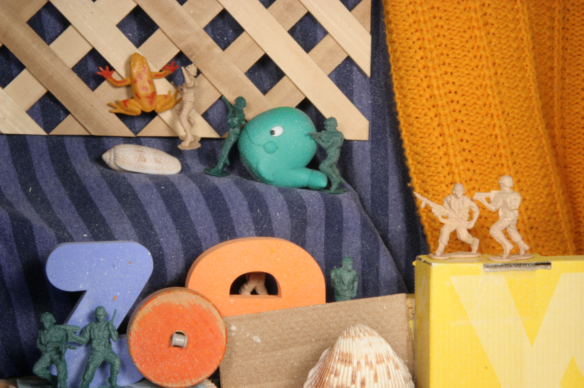
\includegraphics[width=0.1\linewidth]{figures/army/frame10.png}
      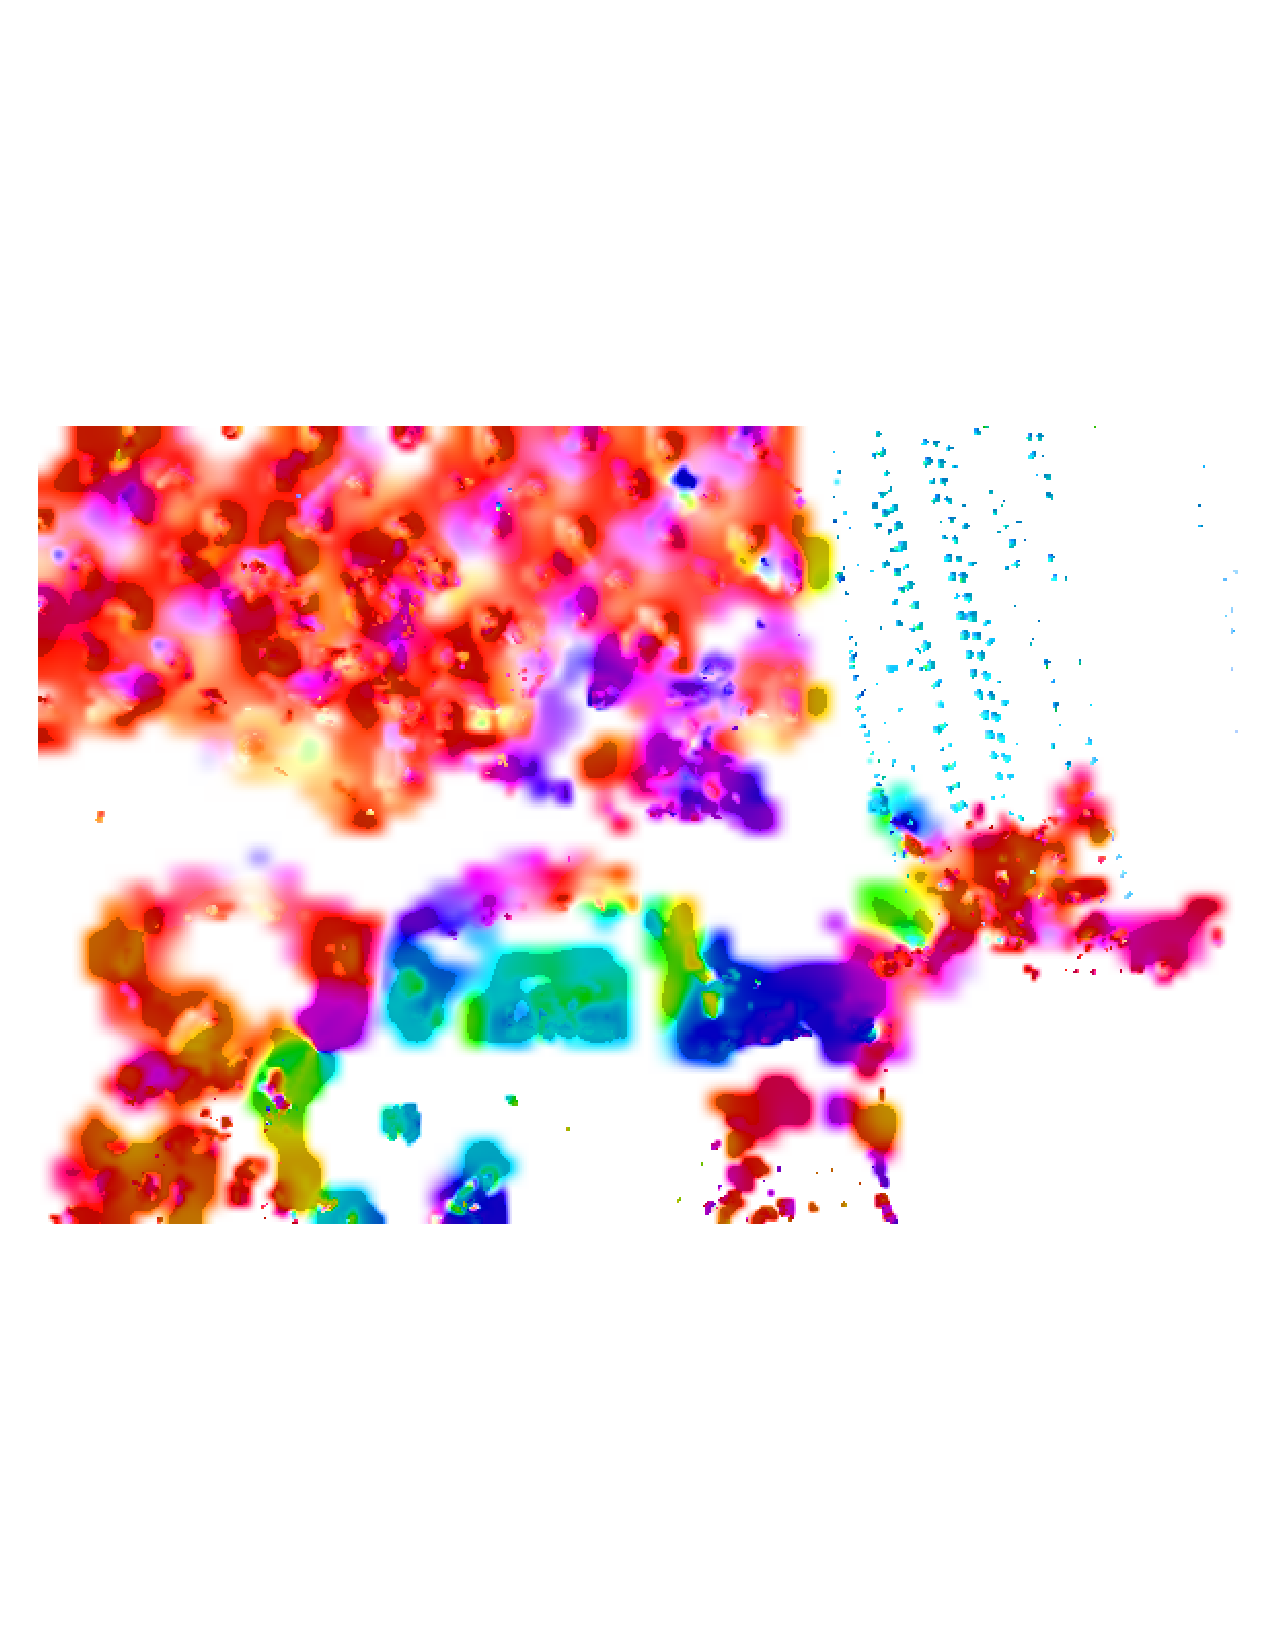
\includegraphics[width=0.1\linewidth]{figures/Army_LK_rgb_pure}
      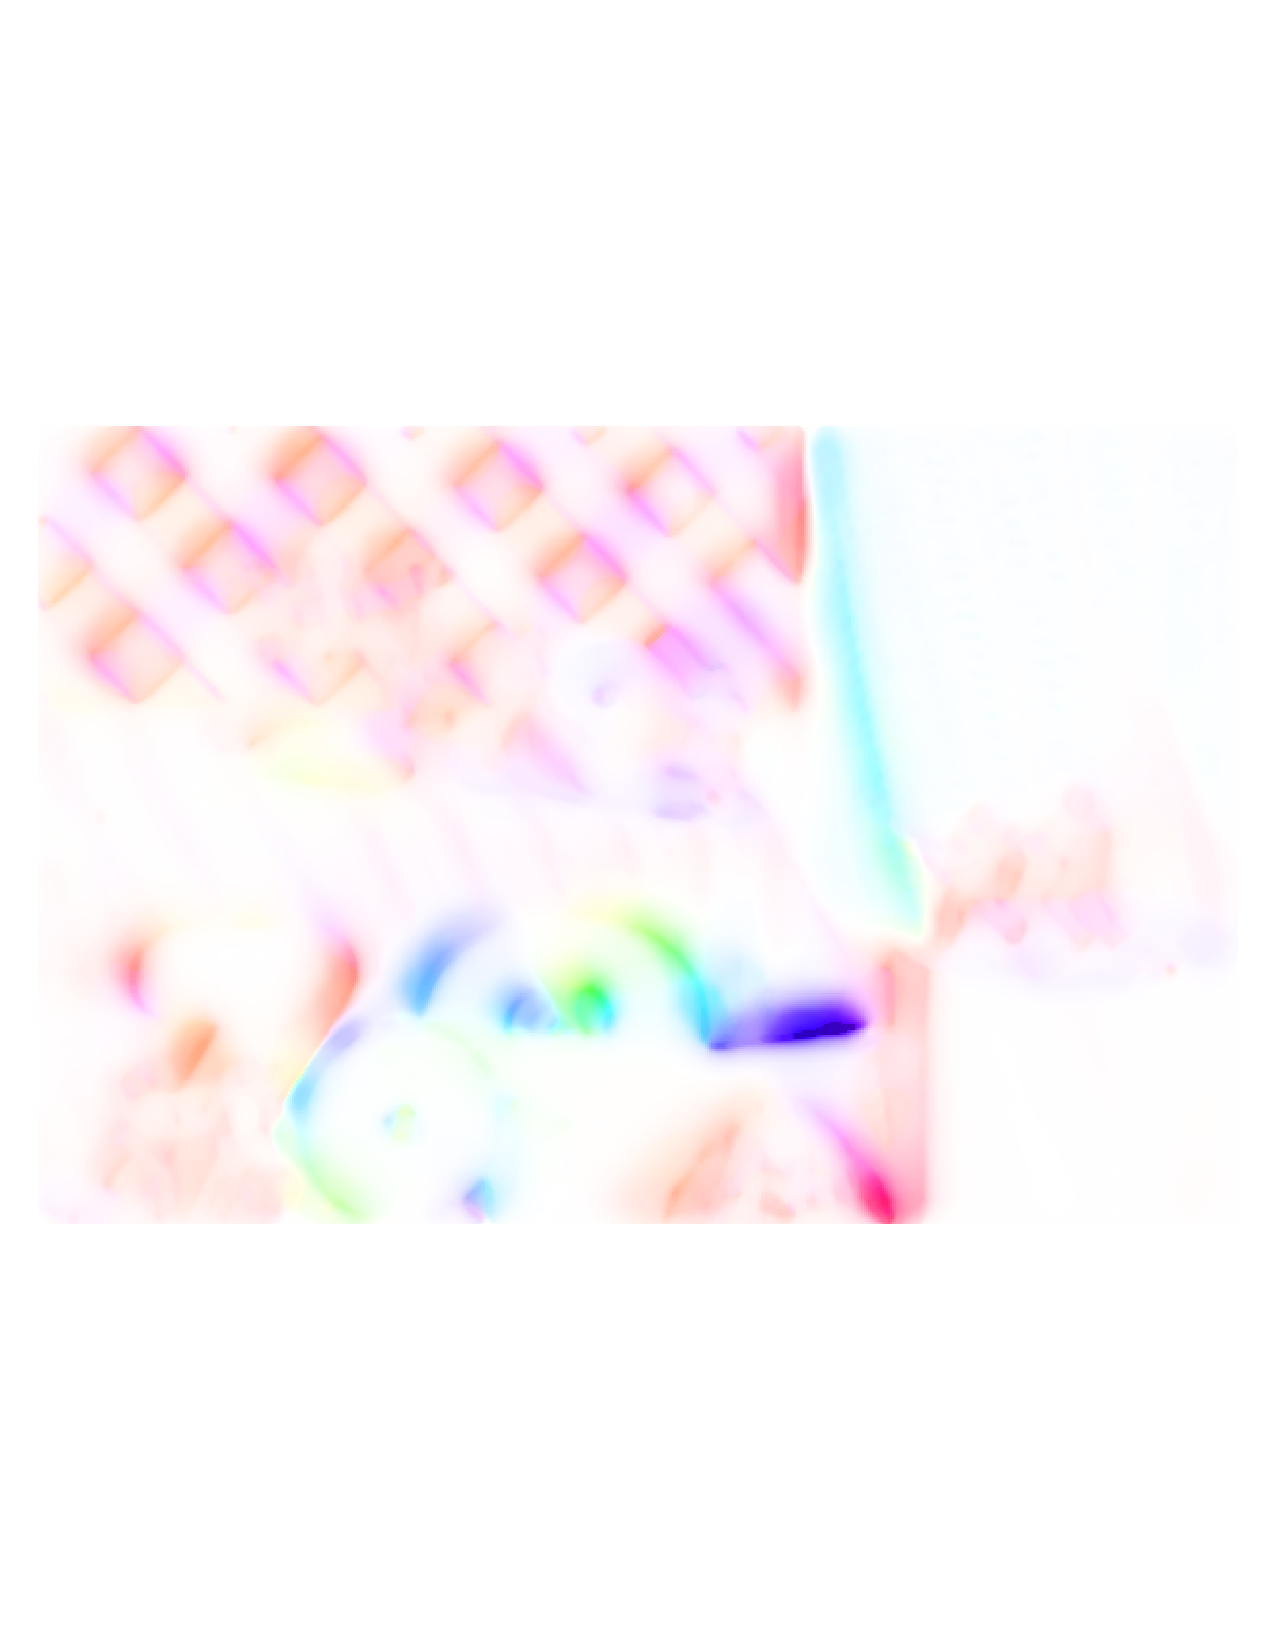
\includegraphics[width=0.1\linewidth]{figures/Army_HS_rgb_pure}
		%\raisebox{-12ex}{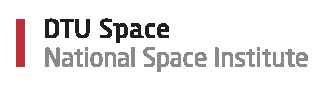
\includegraphics[width=0.15\linewidth]{../logos/tex_dtu_space_b_uk}}
 }
 % Title
 {\sc\Huge Mini-Project for Advanced Image Analysis: Optical Flow Estimation}
 % Authors
 {Xiao Hu\\[0.5em]
 {\texttt{xiahaa@space.dtu.dk}}}
 % University logo
 {
  \begin{tabular}{r}
    
\includegraphics[height=0.08\textheight]{tex_dtu_logo}
  \end{tabular}
 }

%%%%%%%%%%%%%%%%%%%%%%%%%%%%%%%%%%%%%%%%%%%%%%%%%%%%%%%%%%%%%%%%%%%%%%%%%%%%%%
%%% Now define the boxes that make up the poster
%%%---------------------------------------------------------------------------
%%% Each box has a name and can be placed absolutely or relatively.
%%% The only inconvenience is that you can only specify a relative position 
%%% towards an already declared box. So if you have a box attached to the 
%%% bottom, one to the top and a third one which should be inbetween, you 
%%% have to specify the top and bottom boxes before you specify the middle 
%%% box.
%%%%%%%%%%%%%%%%%%%%%%%%%%%%%%%%%%%%%%%%%%%%%%%%%%%%%%%%%%%%%%%%%%%%%%%%%%%%%%

%%%%%%%%%%%%%%%%%%%%%%%%%%%%%%%%%%%%%%%%%%%%%%%%%%%%%%%%%%%%%%%%%%%%%%%%%%%%%%
  \headerbox{Introduction: Optical Flow}{name=contribution,column=0,row=0,span=2}{
%%%%%%%%%%%%%%%%%%%%%%%%%%%%%%%%%%%%%%%%%%%%%%%%%%%%%%%%%%%%%%%%%%%%%%%%%%%%%%
	Small movements between two consecutive frames can be modeled as \textbf{optical flow}. The problem of \textbf{optical flow estimation} is investigated in this mini-project. The Lucas-Kanade \cite{flow:lucas} and the Horn-Shunck methods~\cite{flow:horns} are applied for optical flow estimation in this project. Estimation results on real images are presented for evaluating their performance. 
  }
%%%%%%%%%%%%%%%%%%%%%%%%%%%%%%%%%%%%%%%%%%%%%%%%%%%%%%%%%%%%%%%%%%%%%%%%%%%%%%
  \headerbox{Background}{name=brc,column=0,row=0,below=contribution}{
	\paragraph{Brightness Constancy Constraint}
  	Optical flow is estimated by determining the local translation between two frames which makes the brightness constancy constraint fulfilled: 
  	$$I(x,y,t)=I(x+\Delta x,y+\Delta y,t+\Delta t)$$
	\paragraph{Small Movement Assumption} the local movement is small, so the brightness constancy constraint is approximated as: $$I_xu + I_yv=-I_t \Rightarrow \mathbf{a}^T \mathbf{u} = \mathbf{b}$$
	%Assuming the local movement is small and expanding 
  	\paragraph{Local Consistency Assumption} neighbouring pixels undertake a same displacement $\mathbf{u}$.
  	\paragraph{Minimization Problem} optimal flow is estimated by solving a minimization problem
  	\begin{align*}
  		\mathbf{u}=\underset{\mathbf{u}}{\text{argmin }}E,\ E=\int{\int}||\mathbf{a}^T\mathbf{u}-\mathbf{b}||^2 dxdy
  	\end{align*}
%  	a linear normal equation $\mathbf{Au}=\mathbf{b}$ can be established by stacking the brightness constancy constraints.
  }
  \vspace{-1cm}  
%%%%%%%%%%%%%%%%%%%%%%%%%%%%%%%%%%%%%%%%%%%%%%%%%%%%%%%%%%%%%%%%%%%%%%%%%%%%%%
 \headerbox{Lucas-Kanade Method}{name=lk,column=0,row=0,below=brc}{
  Solve with least-square solution
  \begin{align*}
  \mathbf{u} = (\mathbf{A}^T\mathbf{A})^{-1}\mathbf{A}^T\mathbf{b},\ \mathbf{A}=[\mathbf{a}_1, \cdots, \mathbf{a}_k]^T
  \end{align*}
  }
   \headerbox{Horn-Shunck Method}{name=hs,column=0,row=0,above=bottom}{
	Add regularization on the smoothness of the flow and solve a joint minimization problem
  \begin{align*}
  E_{joint} = E+\int{\int}\alpha^2(||\bigtriangledown u||^2+||\bigtriangledown v||^2) dxdy
  \end{align*}
  The optimization problem is solved iteratively
  \begin{align*}
  u^{k+1}=\bar{u}^k-\frac{I_x(I_x\bar{u}^k+I_y\bar{v}^k+I_t)}{\alpha^2+I_x^2+I_y^2}\\
  v^{k+1}=\bar{v}^k-\frac{I_y(I_x\bar{u}^k+I_y\bar{v}^k+I_t)}{\alpha^2+I_x^2+I_y^2}
  \end{align*}
  }
%%%%%%%%%%%%%%%%%%%%%%%%%%%%%%%%%%%%%%%%%%%%%%%%%%%%%%%%%%%%%%%%%%%%%%%%%%%%%%
\headerbox{Implementation}{name=lowrestracking,column=1,span=1,below=speed,below=contribution}{
\paragraph{Conditioning} $\mathbf{Au=b}$ may be ill-posed. To deal with:
\begin{itemize}
\item check the harmonic mean: $\frac{\text{det}(\mathbf{A})}{\text{tr}(\mathbf{A})} > \tau$.
\item check the minimum eigenvalue: $\lambda_{min}> \tau$.
\end{itemize}
\paragraph{Gradient Kernel} To compute $I_x, I_y$, different kernels are applied:
\begin{itemize}
\item $[-1,0,1]$.
\item Derivative of Gaussian.
\end{itemize}
\paragraph{Weighting Kernel} To sum up the contributions from neighbouring pixels, the following kernels are applied:
\begin{itemize}
\item Box filter.
\item Gaussian Kernel.
\end{itemize}
\paragraph{Coarse-to-Fine} To deal with large movement, image pyramid is used to establish a coarse-to-fine flow estimation.
\newline
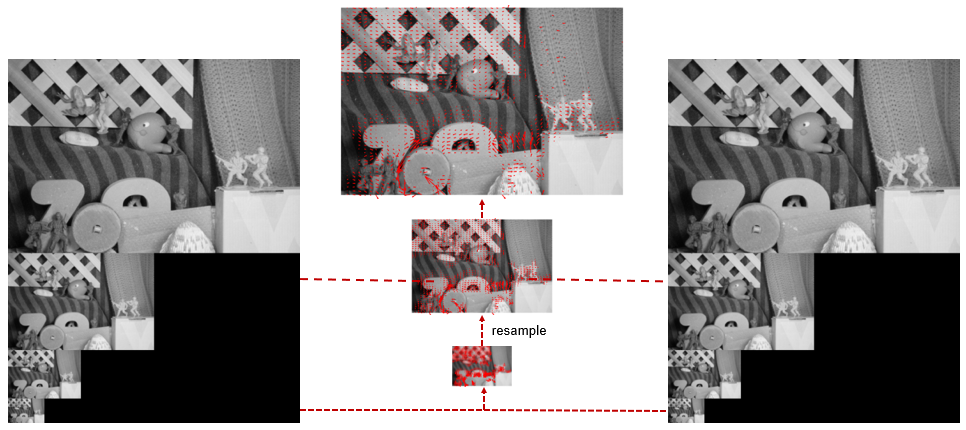
\includegraphics[width=1\linewidth]{figures/final.png}%
\vspace{0.25em}
\textbf{Coarse-to-Fine Optical Flow Estimation}.
}
 %%%%%%%%%%%%%%%%%%%%%%%%%%%%%%%%%%%%%%%%%%%%%%%%%%%%%%%%%%%%%%%%%%%%%%%%%%%%%%
   \headerbox{Results}{name=speed,column=2,row=0,span=2}{
 %%%%%%%%%%%%%%%%%%%%%%%%%%%%%%%%%%%%%%%%%%%%%%%%%%%%%%%%%%%%%%%%%%%%%%%%%%%%%%
  \begin{tabular}{c@{\hspace{0.05em}}c@{\hspace{0.2em}}c@{\hspace{0.1em}}c@{\hspace{0.2em}}c@{\hspace{0.1em}}c@{\hspace{0.1em}}c}
   \multicolumn{6}{c}{\smaller Army} &\\[-0.2em]
%   \multicolumn{2}{c}{\smaller Lucas-Kanade} &
%   \multicolumn{2}{c}{\smaller Horn-Shunck} 
   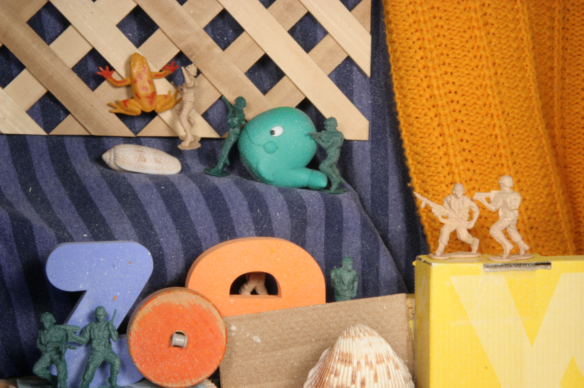
\includegraphics[width=0.16\linewidth]{figures/army/frame10.png}&
   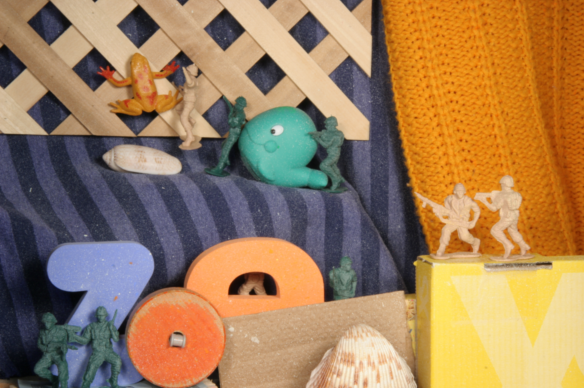
\includegraphics[width=0.16\linewidth]{figures/army/frame11.png}&
   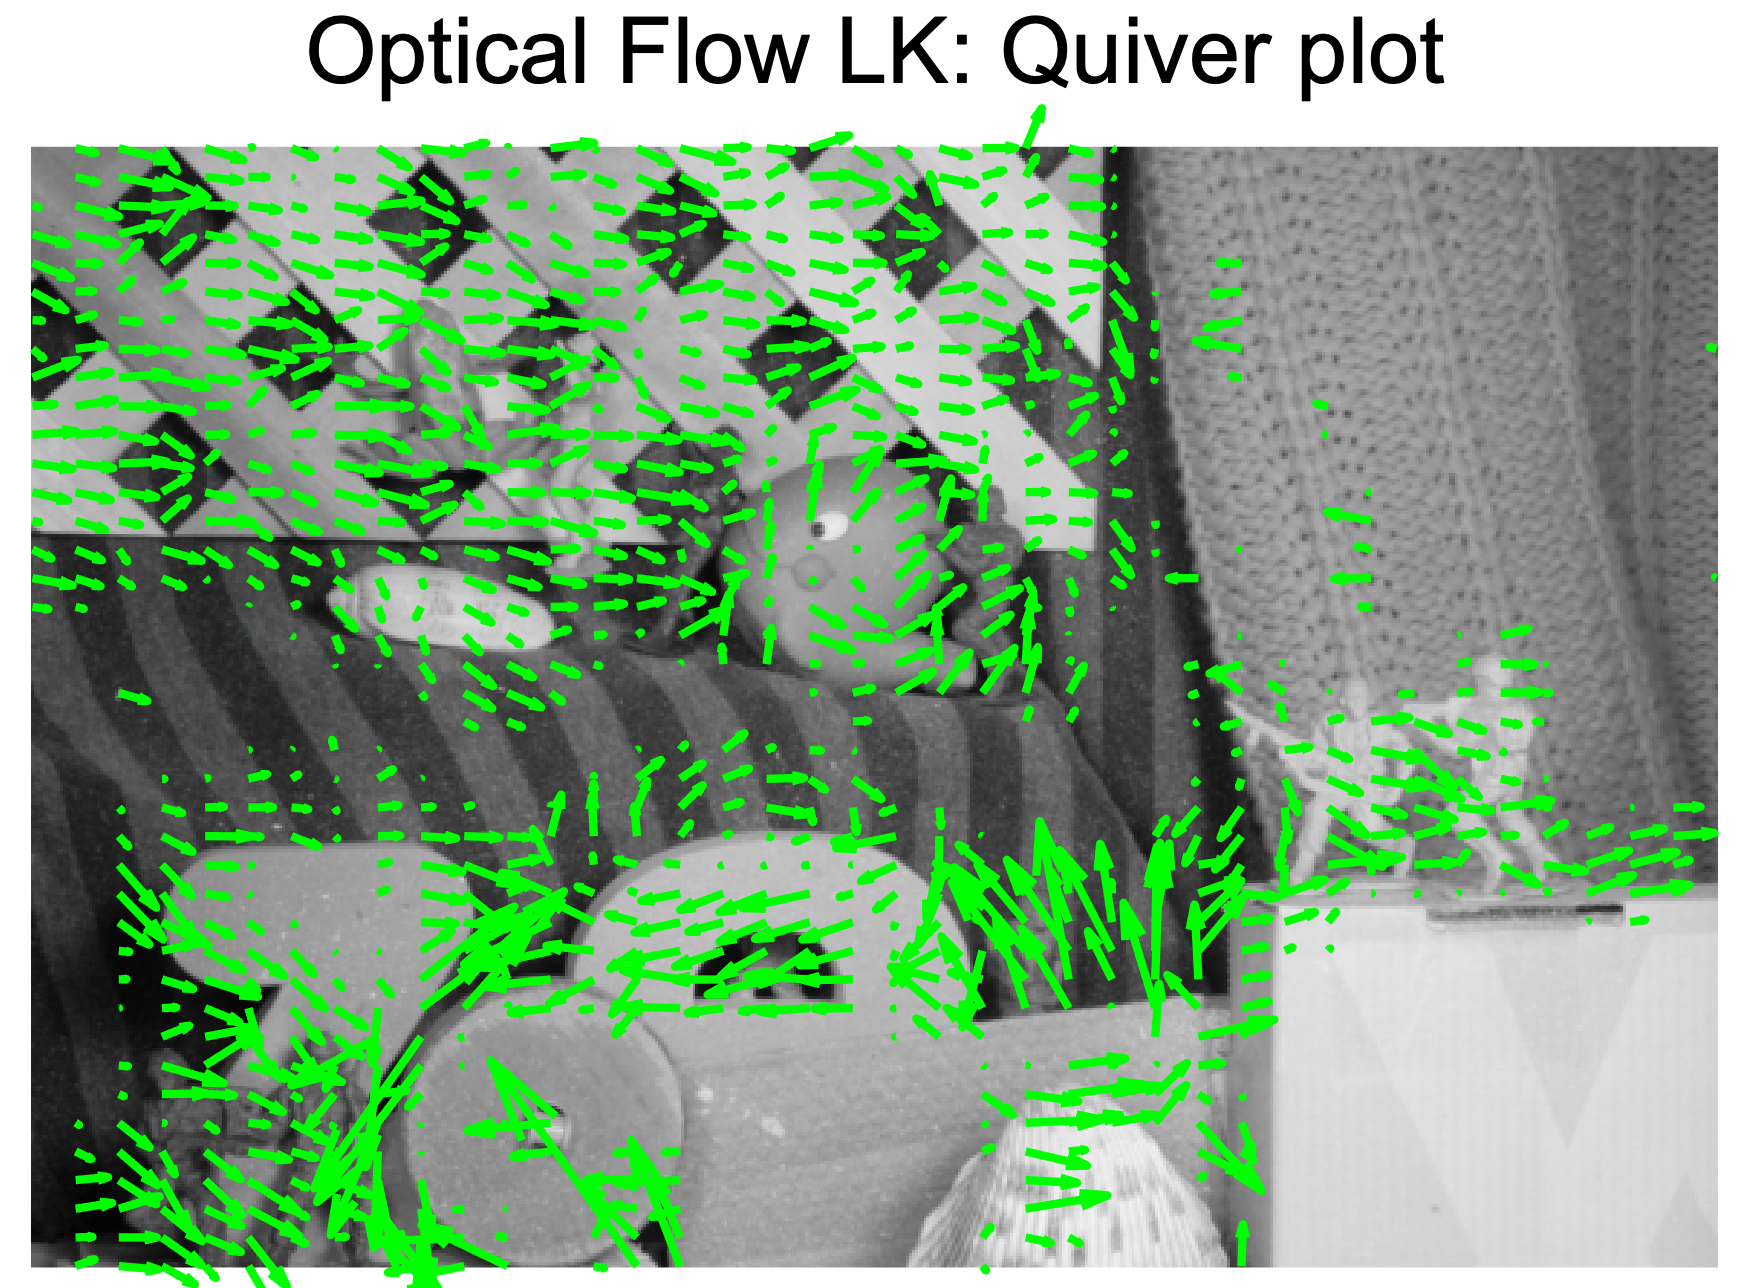
\includegraphics[width=0.16\linewidth]{figures/army/Army_LK_quiver.png}&
   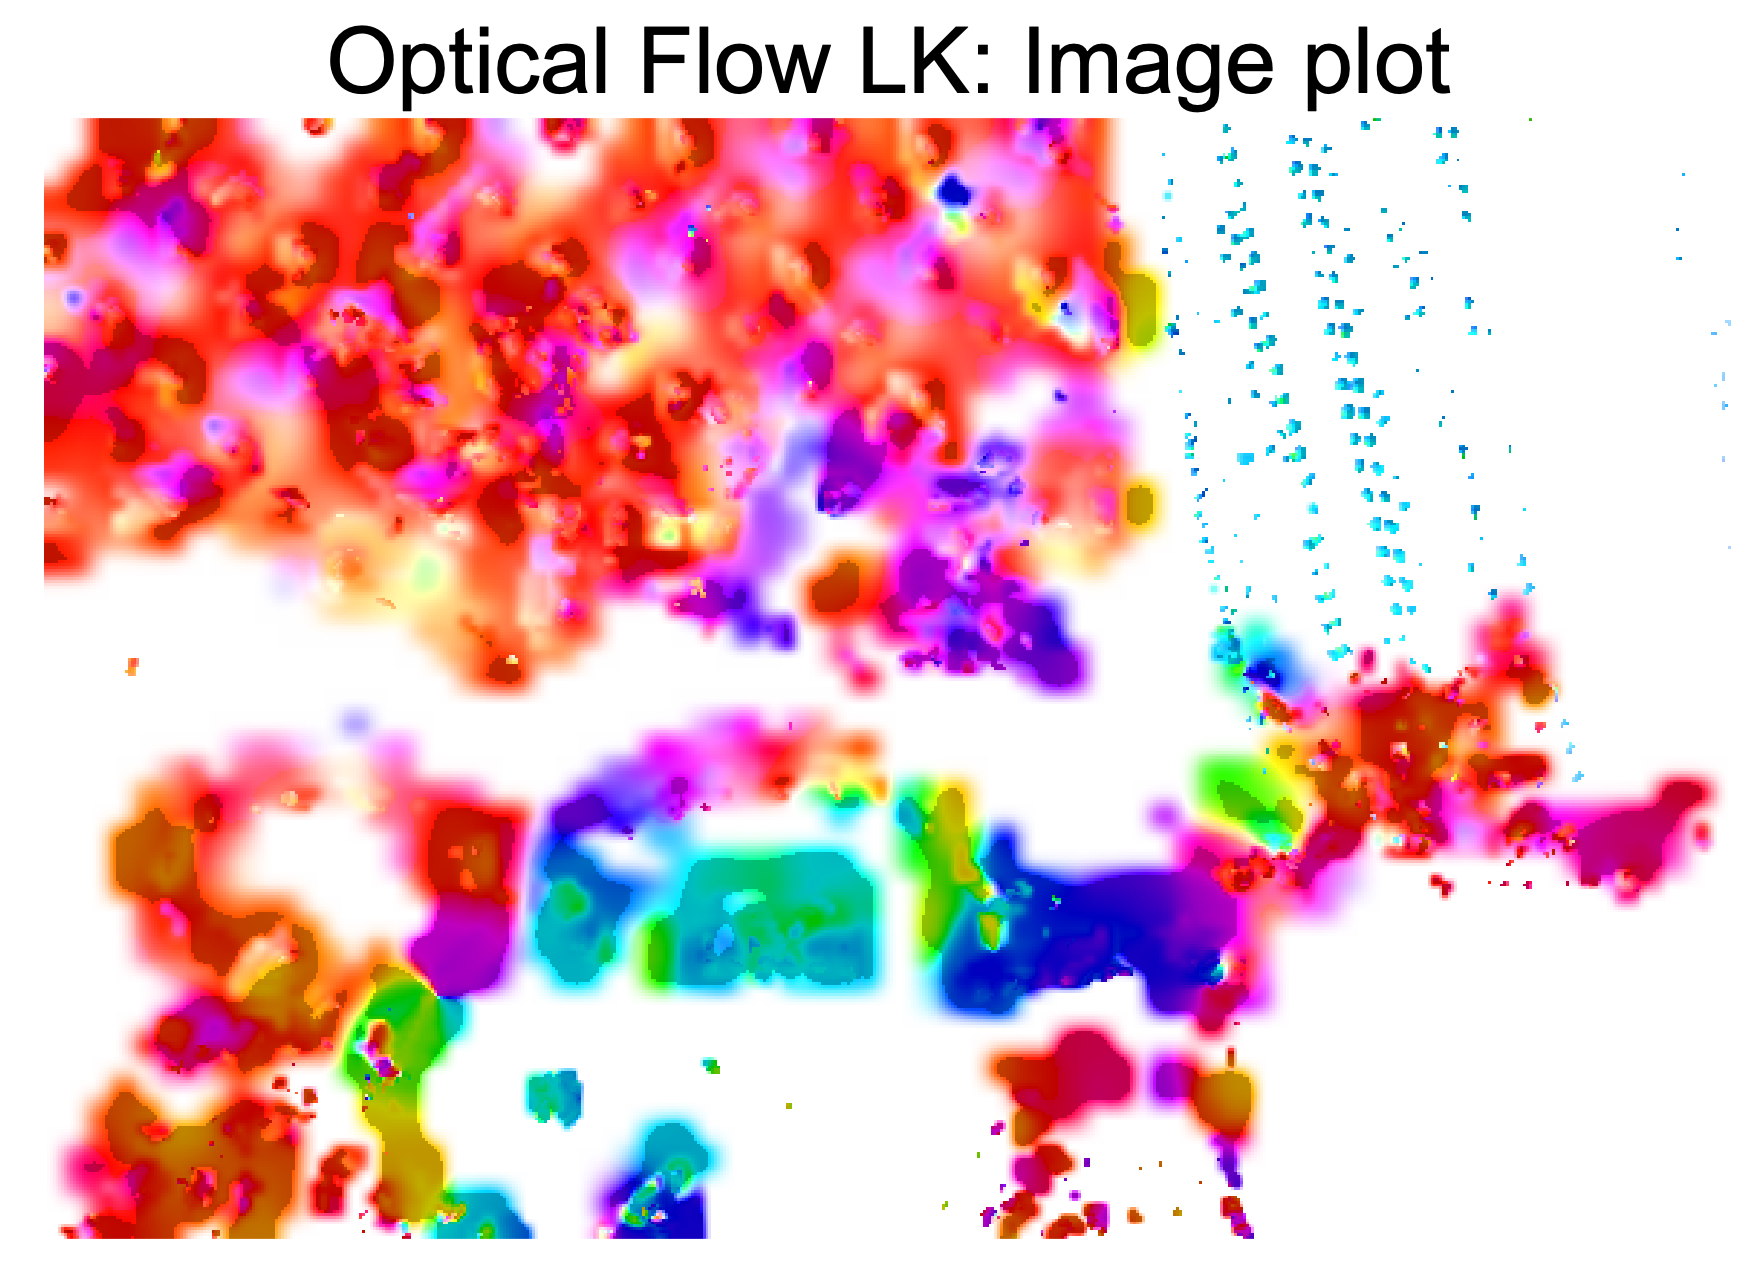
\includegraphics[width=0.16\linewidth]{figures/army/Army_LK_rgb.png}&
   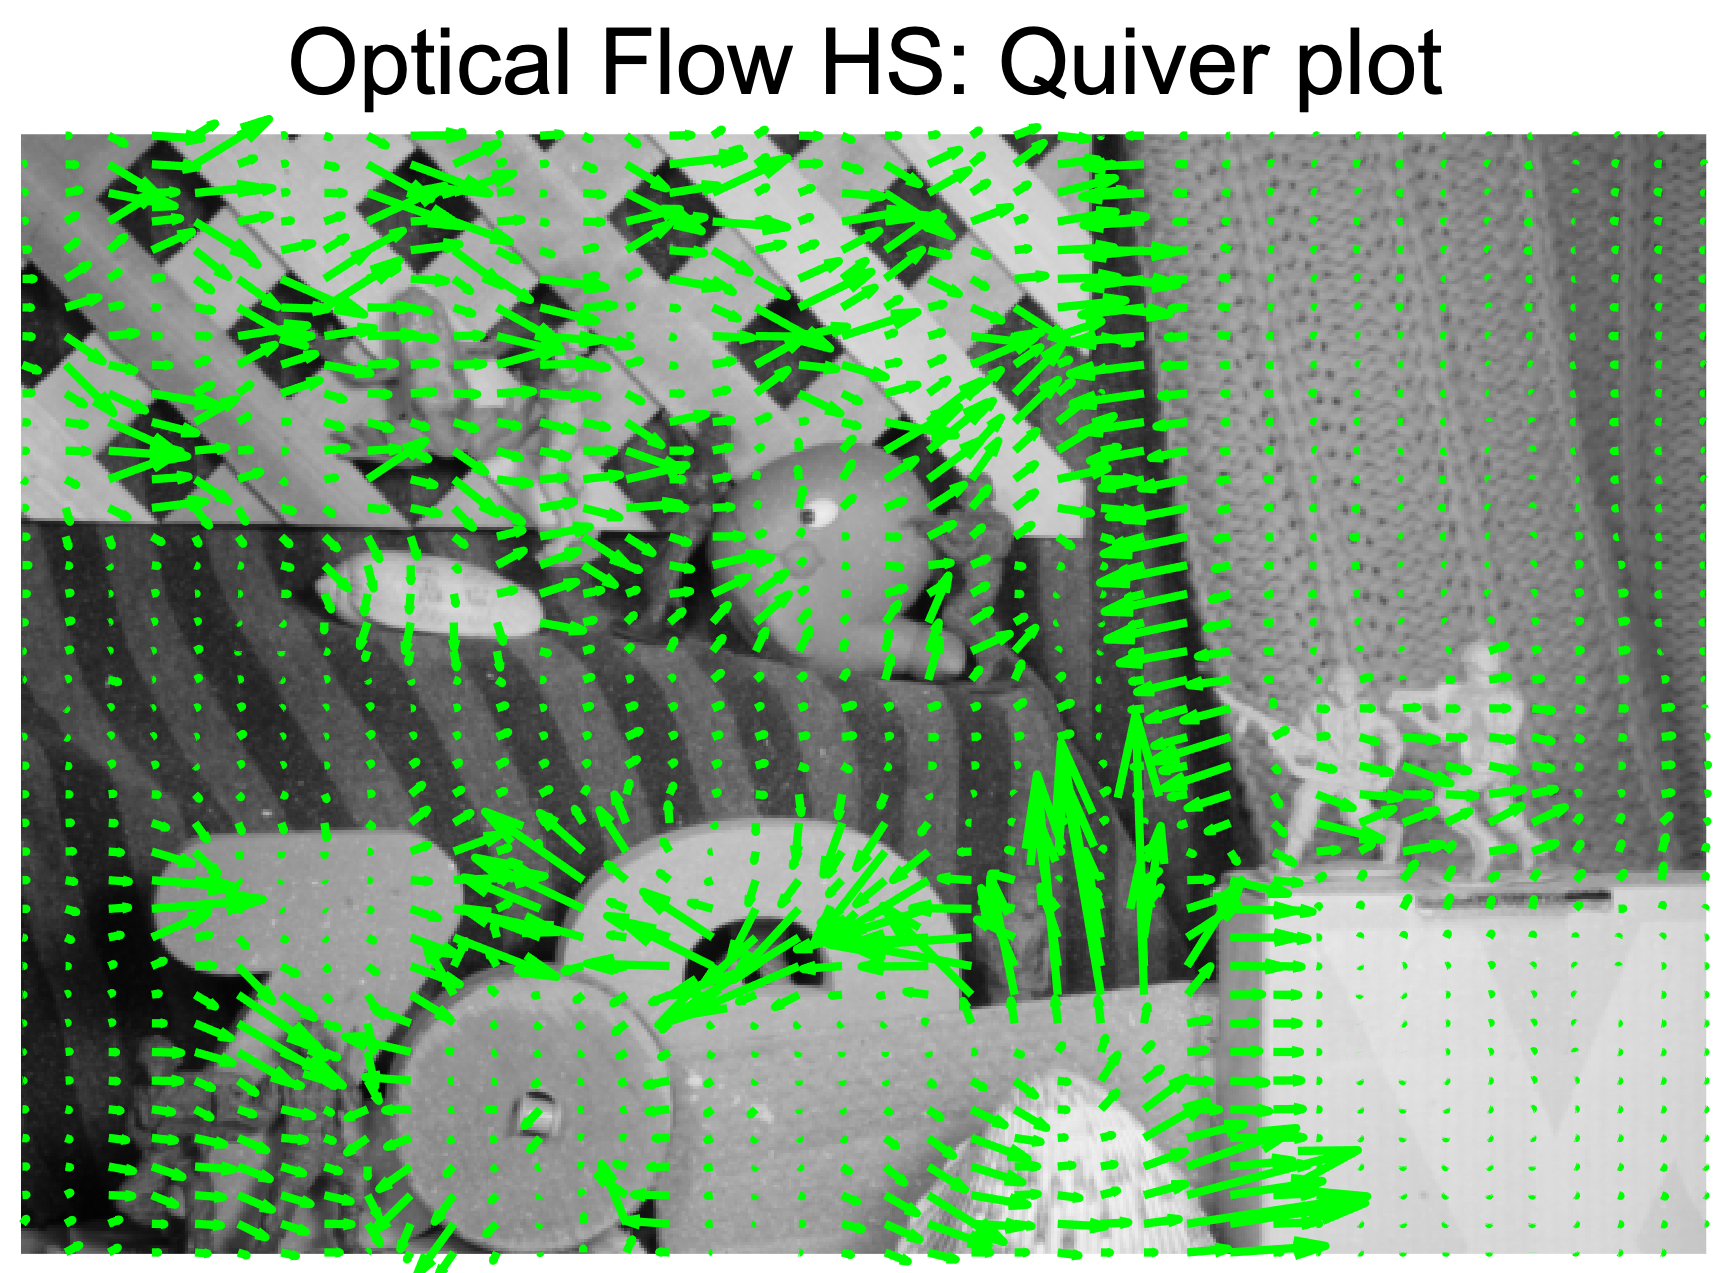
\includegraphics[width=0.16\linewidth]{figures/army/Army_HS_quiver.png}&
   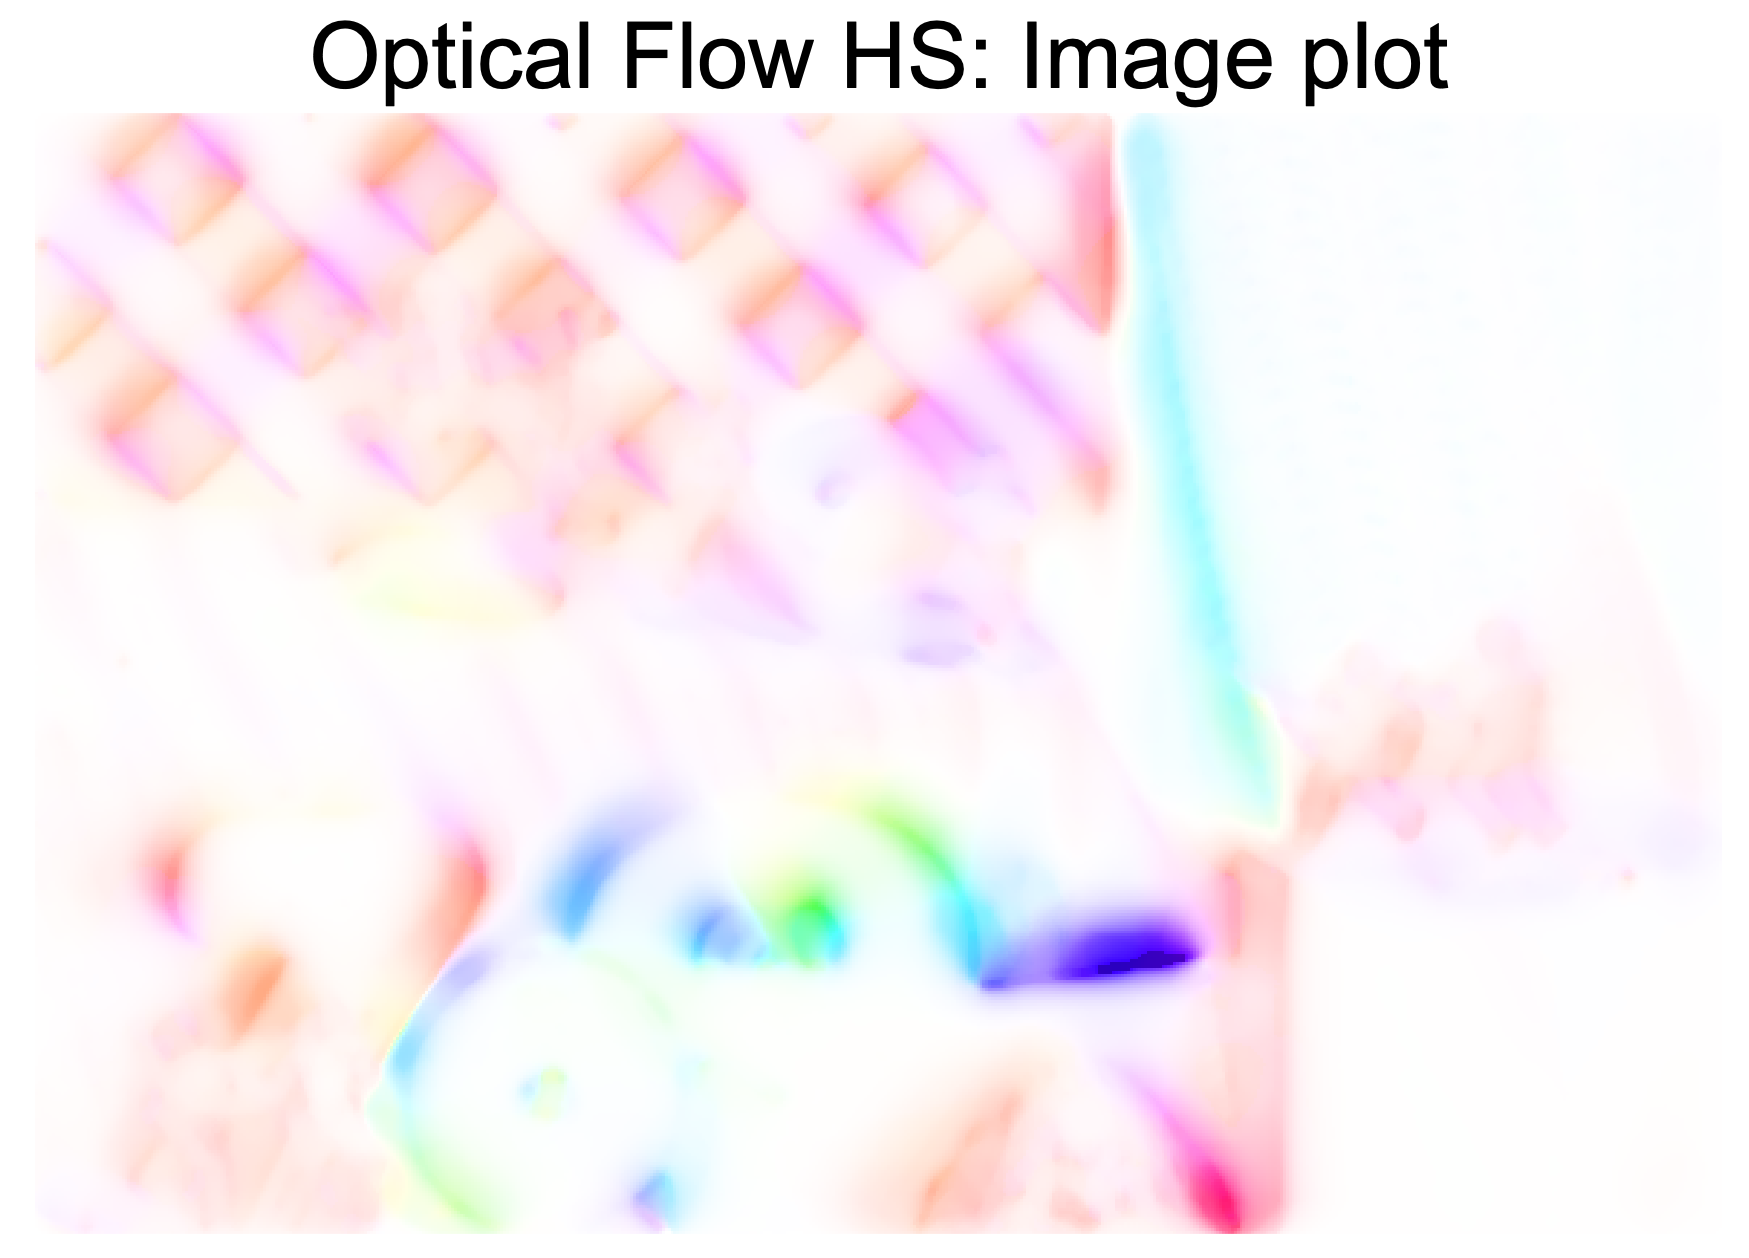
\includegraphics[width=0.16\linewidth]{figures/army/Army_HS_rgb.png}\\[-0.1em]
   %
   \multicolumn{6}{c}{\smaller Teddy} &\\[-0.2em]
   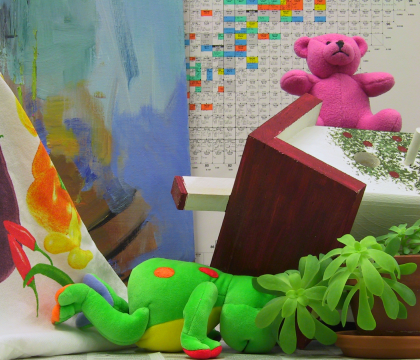
\includegraphics[width=0.16\linewidth]{figures/Teddy/frame10.png}&
   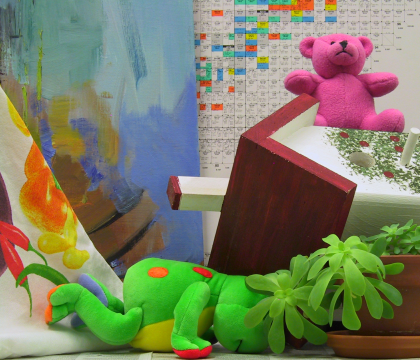
\includegraphics[width=0.16\linewidth]{figures/Teddy/frame11.png}&
   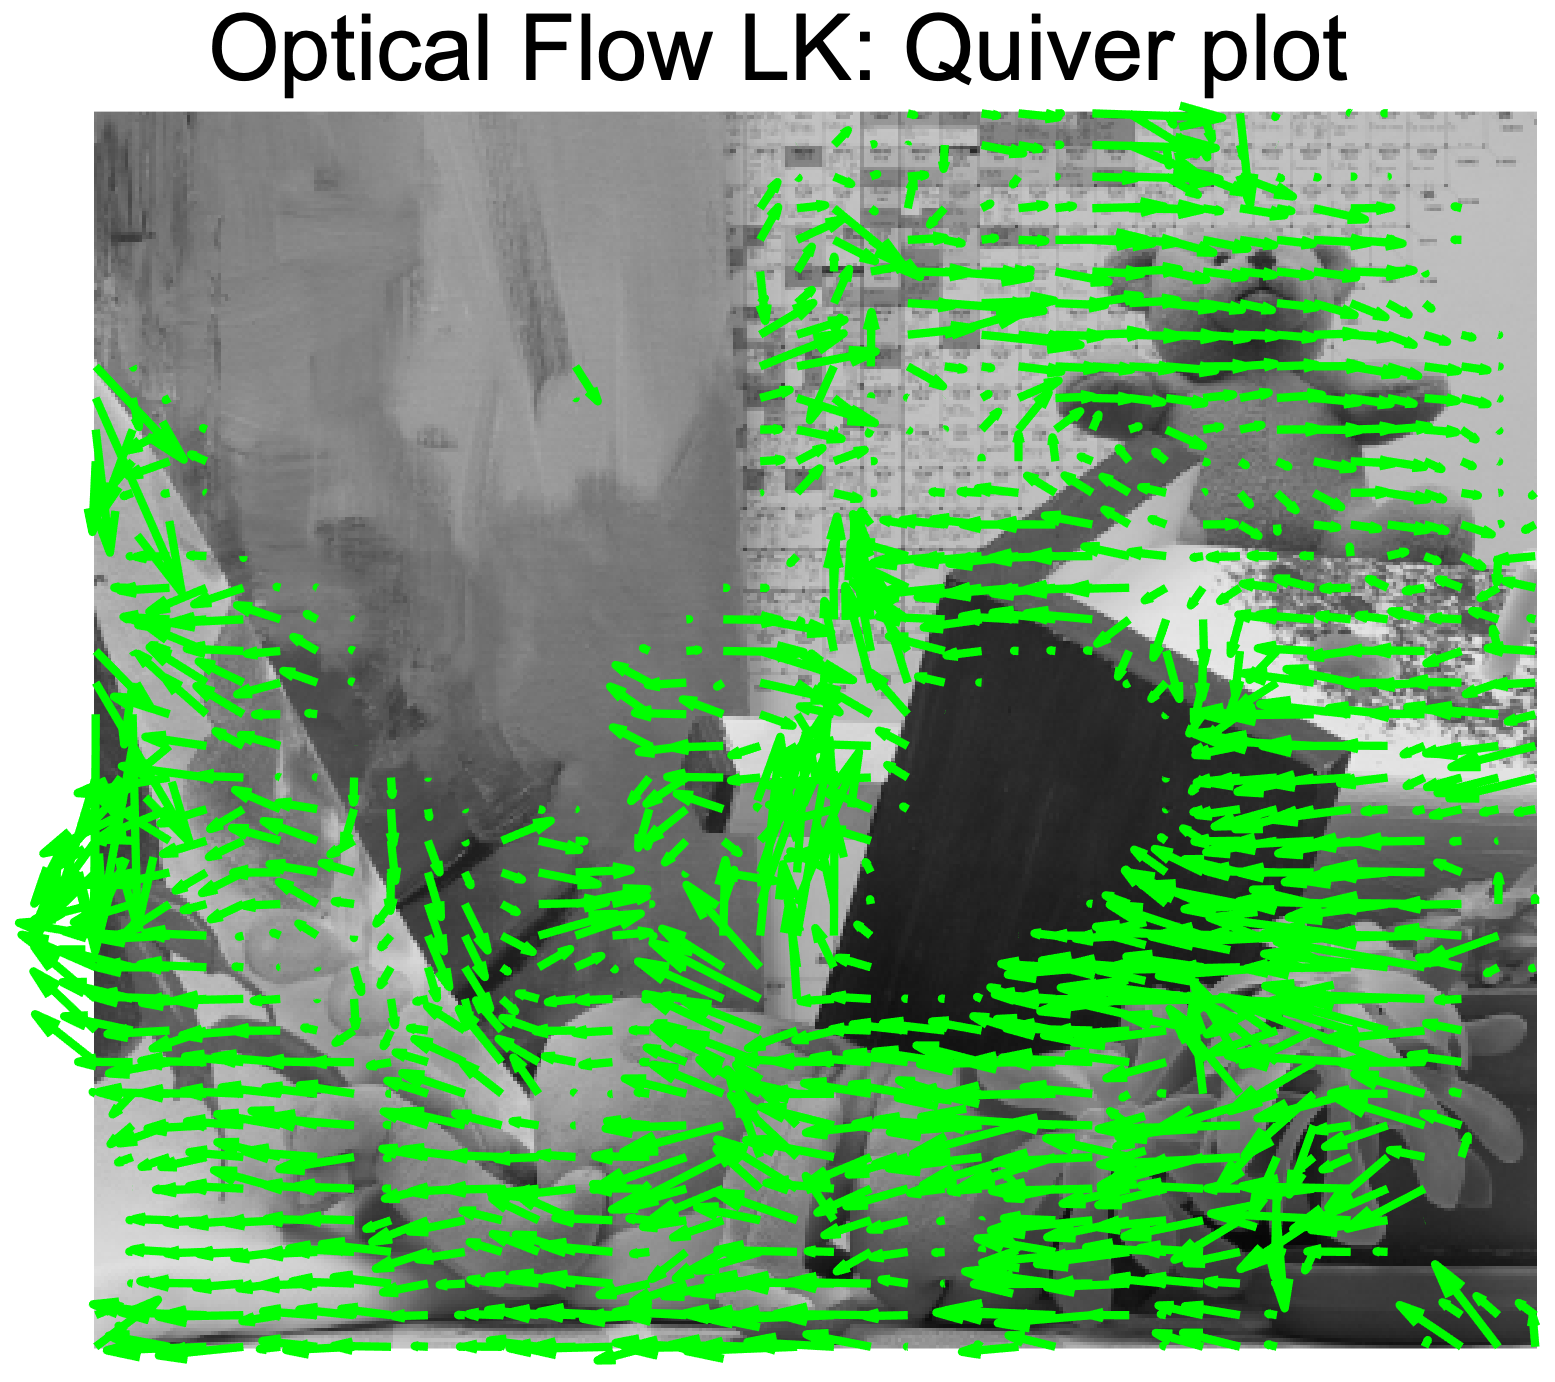
\includegraphics[width=0.16\linewidth]{figures/Teddy/Teddy_LK_quiver.png}&
   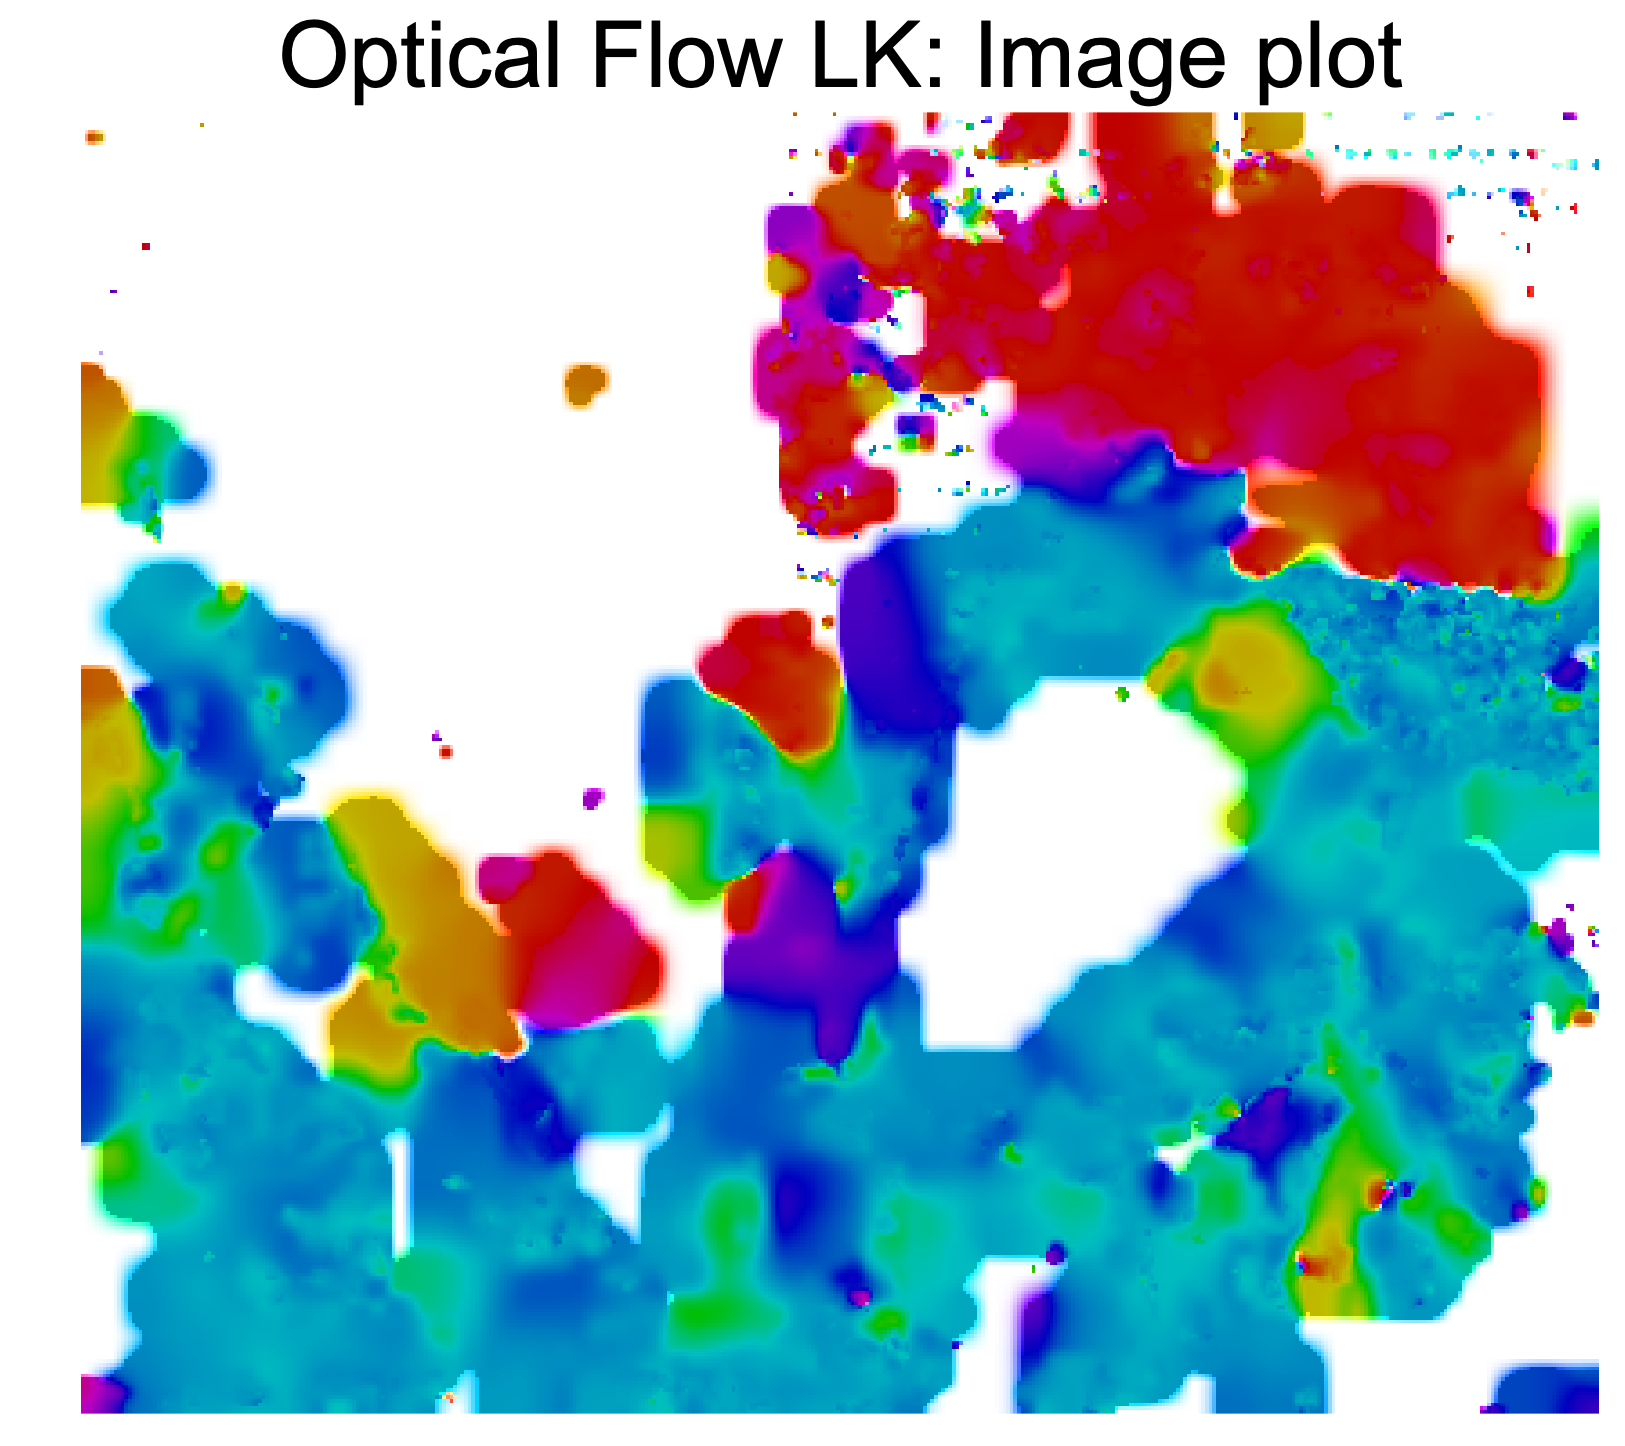
\includegraphics[width=0.16\linewidth]{figures/Teddy/Teddy_LK_rgb.png}&
   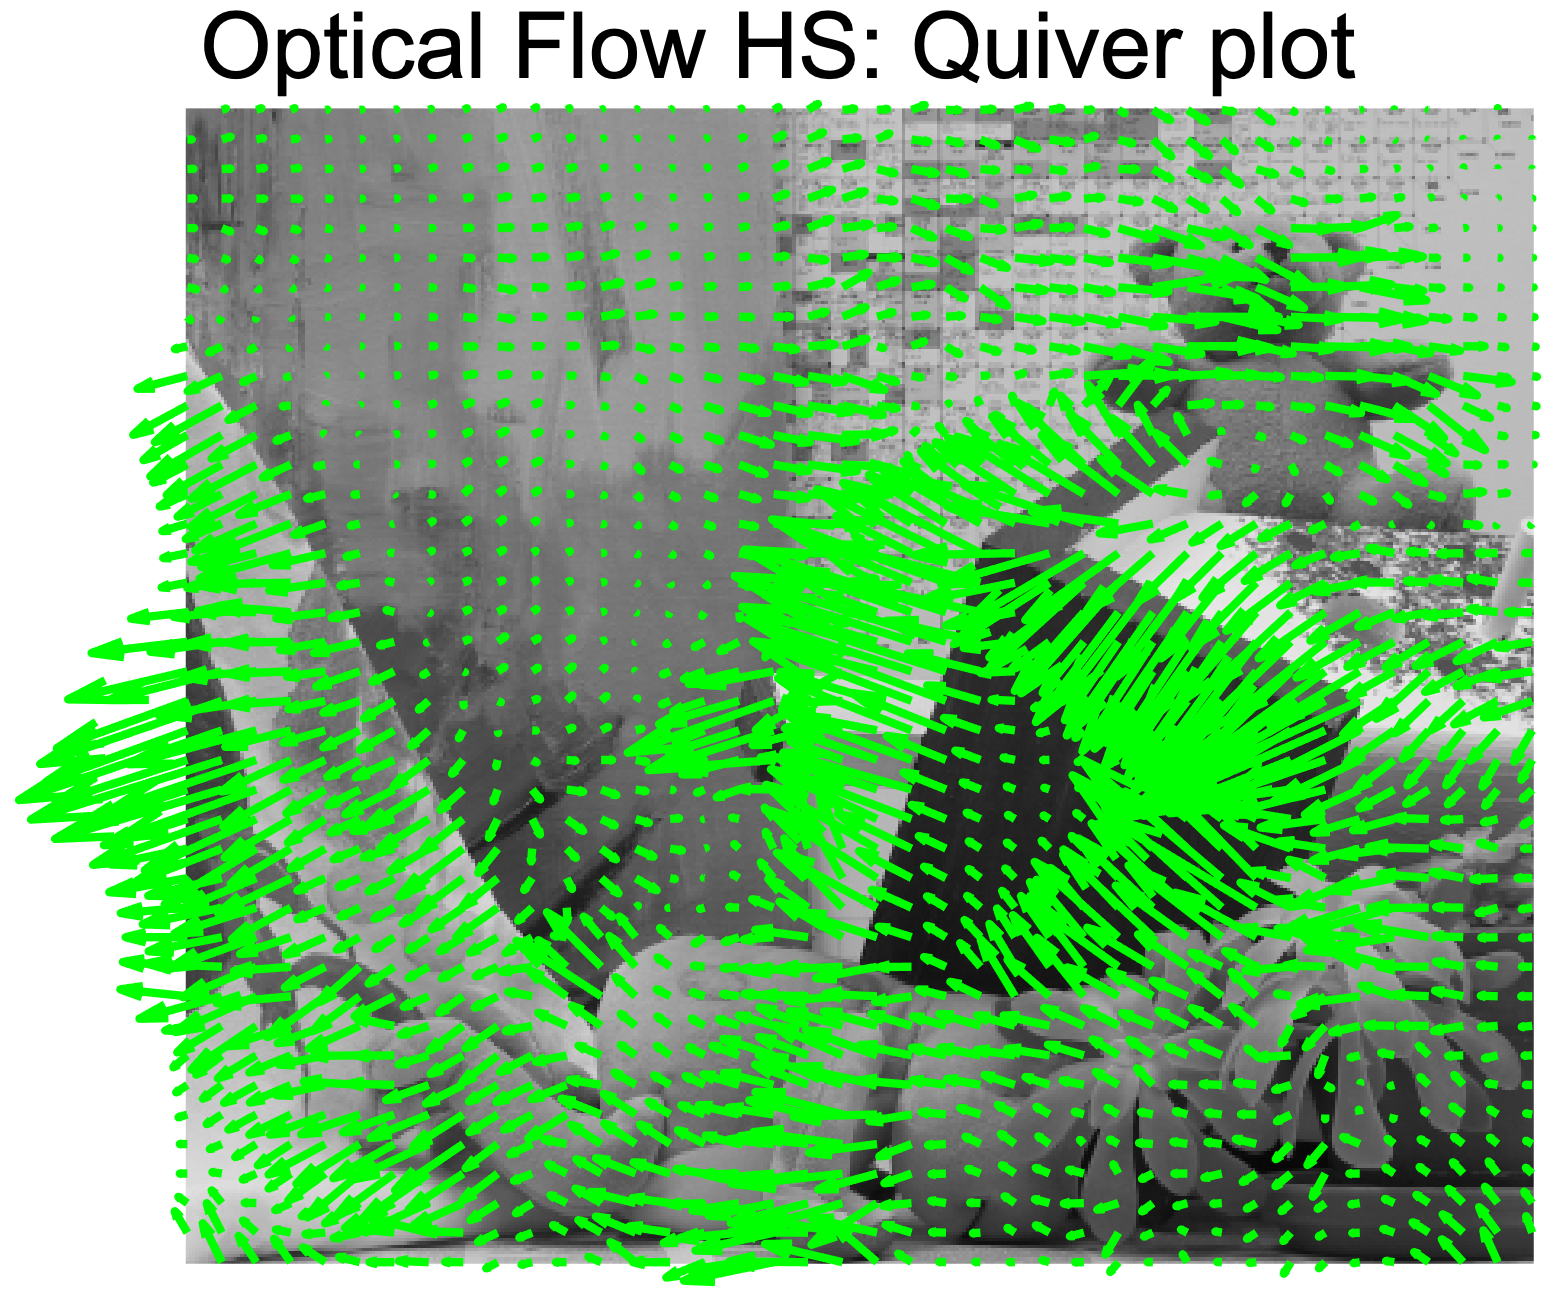
\includegraphics[width=0.16\linewidth]{figures/Teddy/Teddy_HS_quiver.png}&
   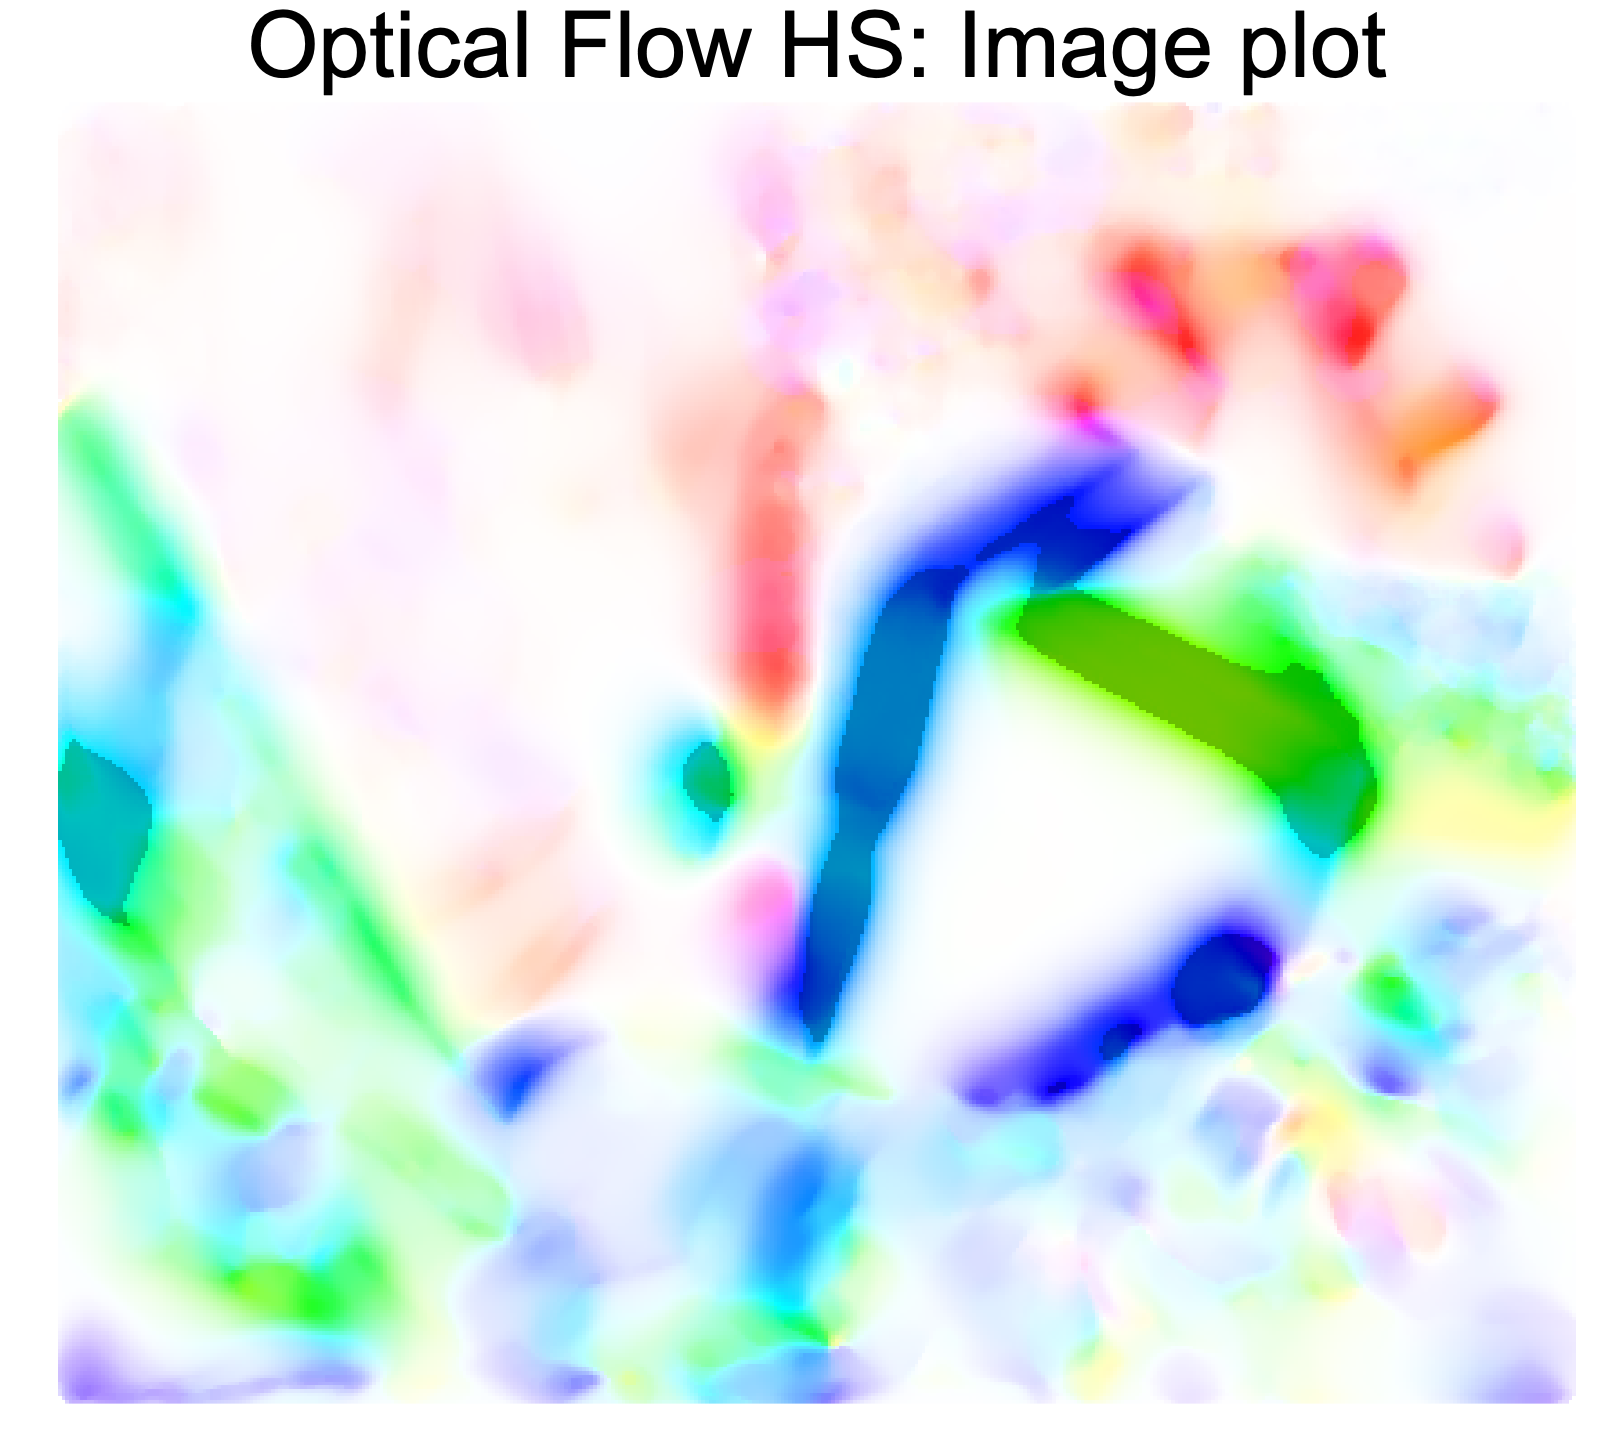
\includegraphics[width=0.16\linewidth]{figures/Teddy/Teddy_HS_rgb.png}\\[-0.1em]
   %
   \multicolumn{6}{c}{\smaller Basketball} &\\[-0.2em]
   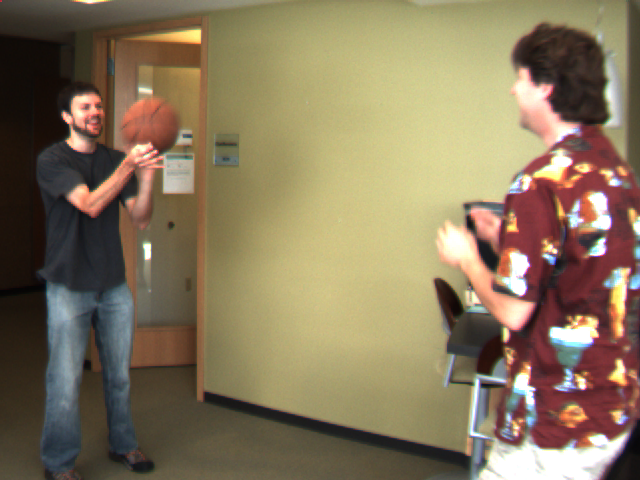
\includegraphics[width=0.16\linewidth]{figures/basketball/frame10.png}&
   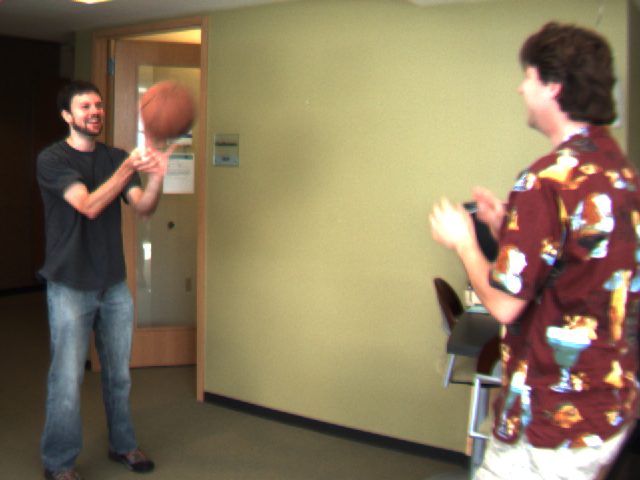
\includegraphics[width=0.16\linewidth]{figures/basketball/frame11.png}&
   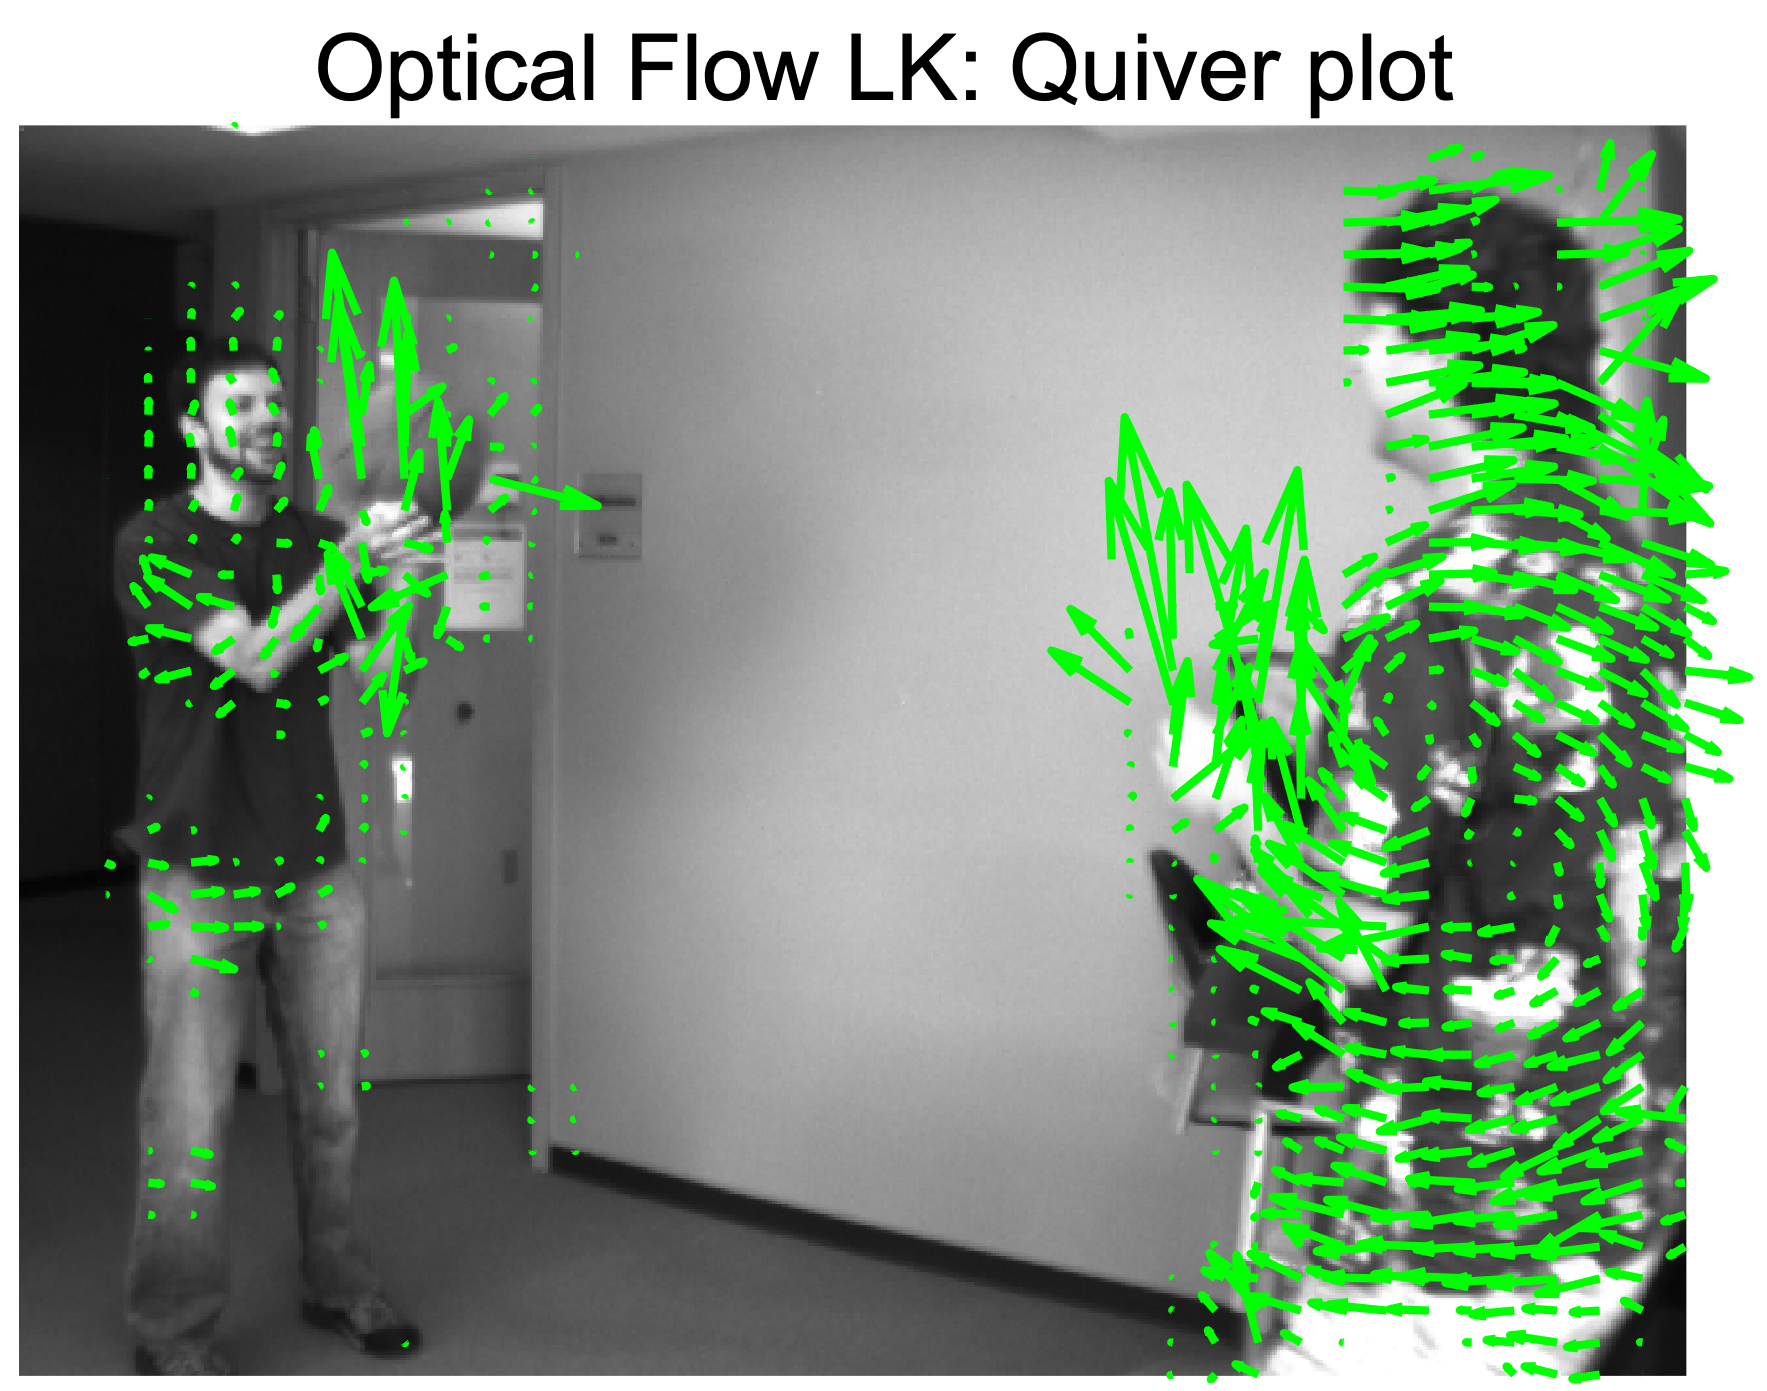
\includegraphics[width=0.16\linewidth]{figures/basketball/Basketball_LK_quiver.png}&
   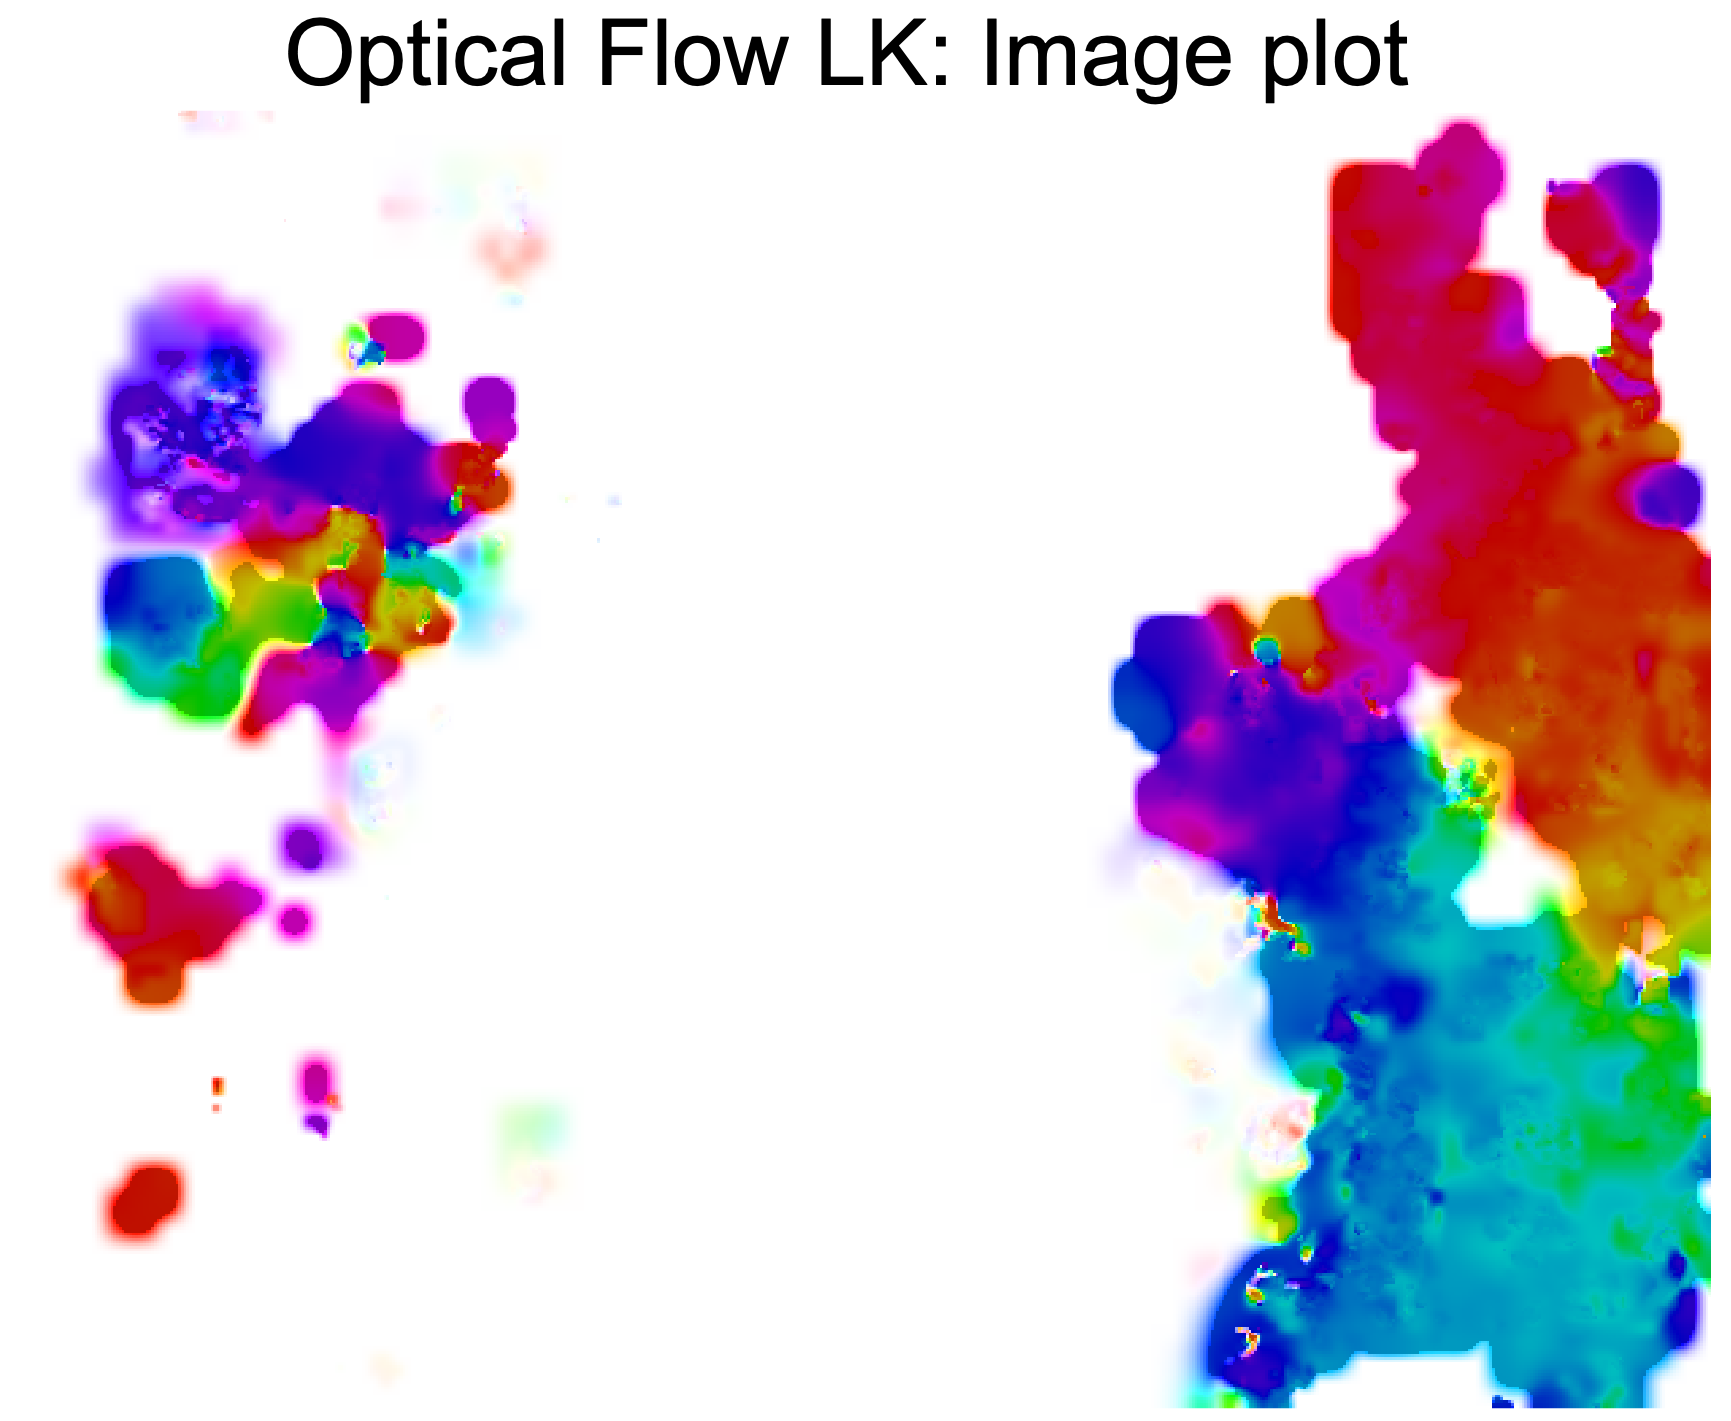
\includegraphics[width=0.16\linewidth]{figures/basketball/Basketball_LK_rgb.png}&
   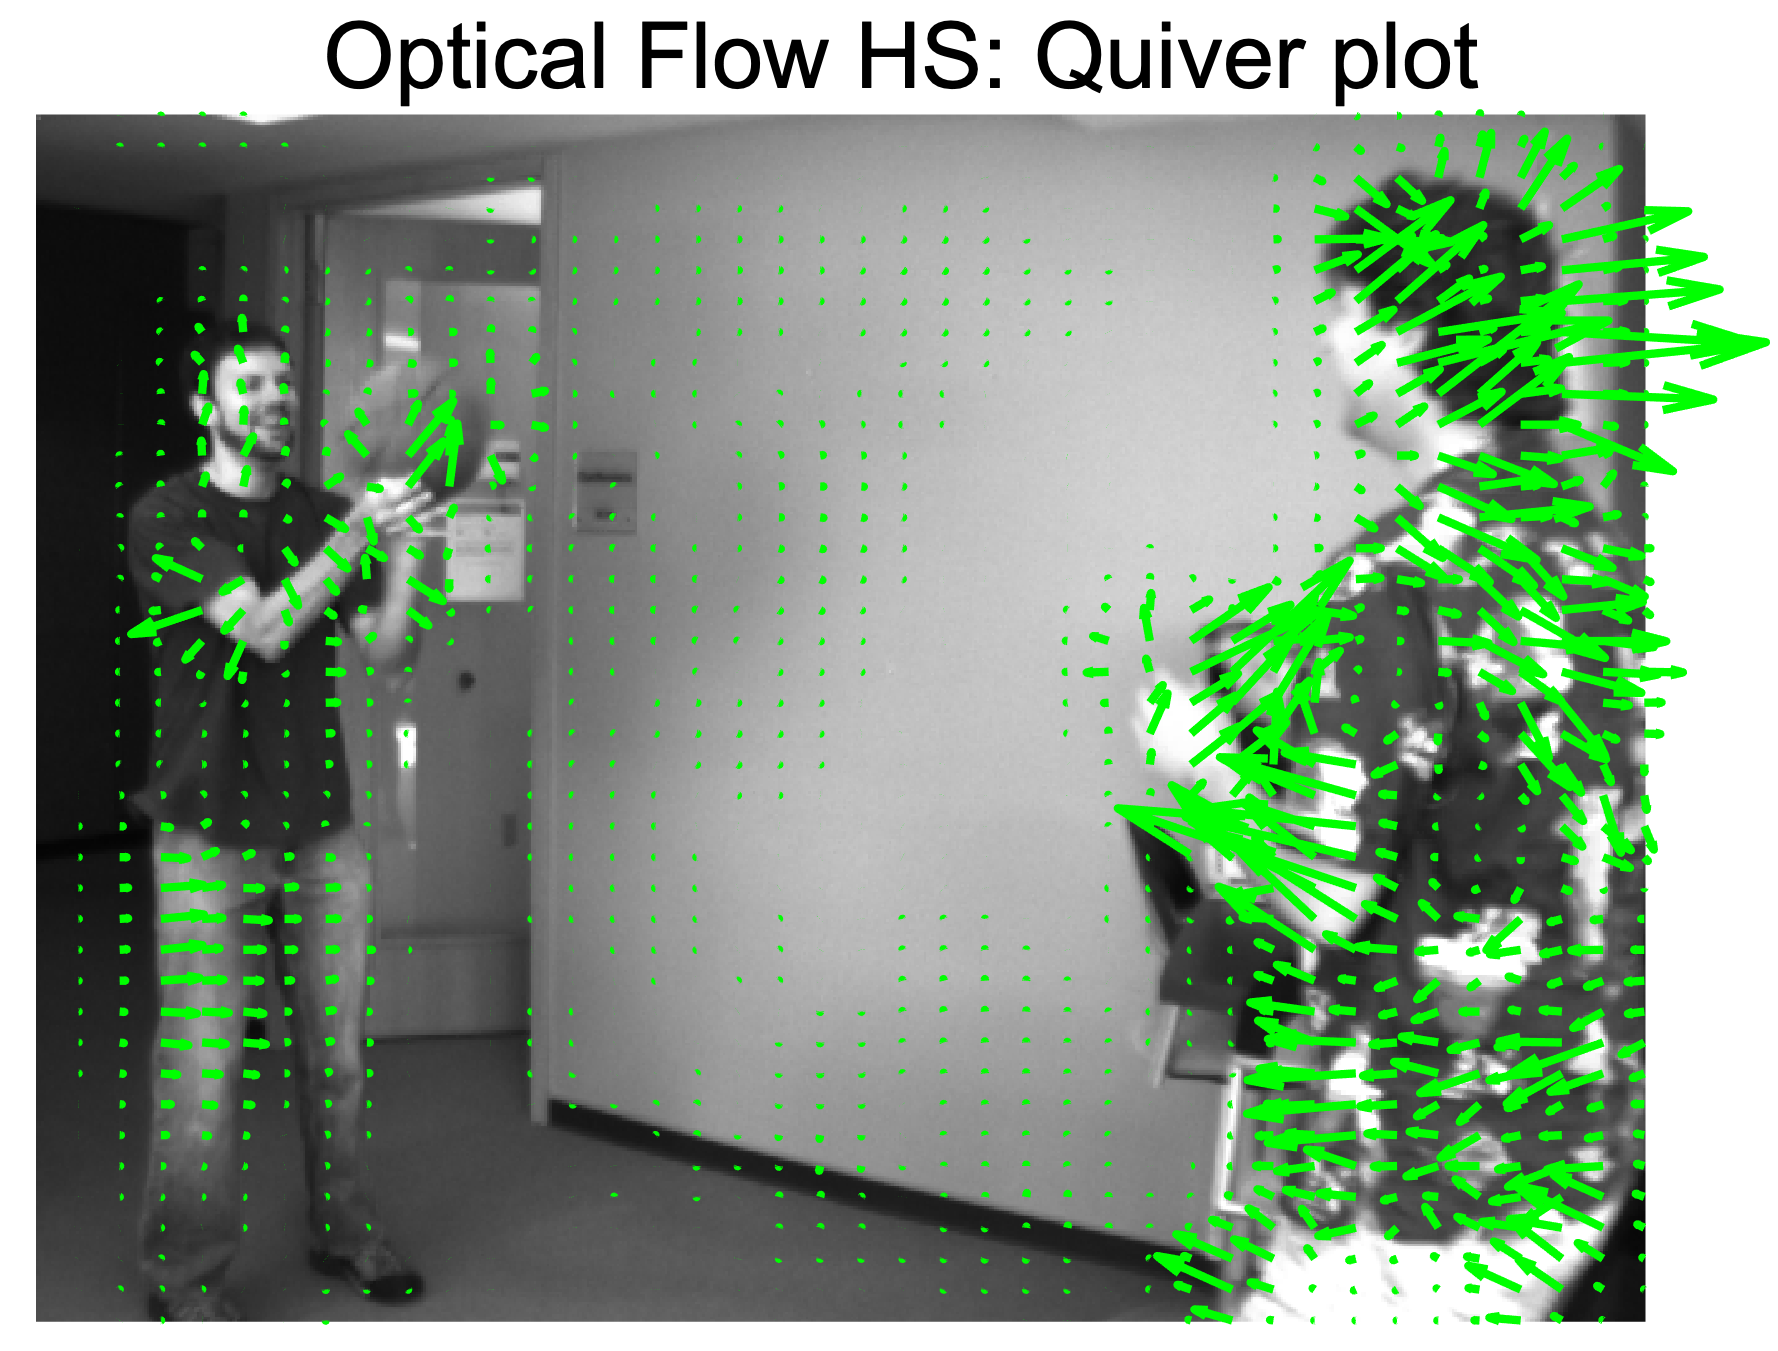
\includegraphics[width=0.16\linewidth]{figures/basketball/Basketball_HS_quiver.png}&
   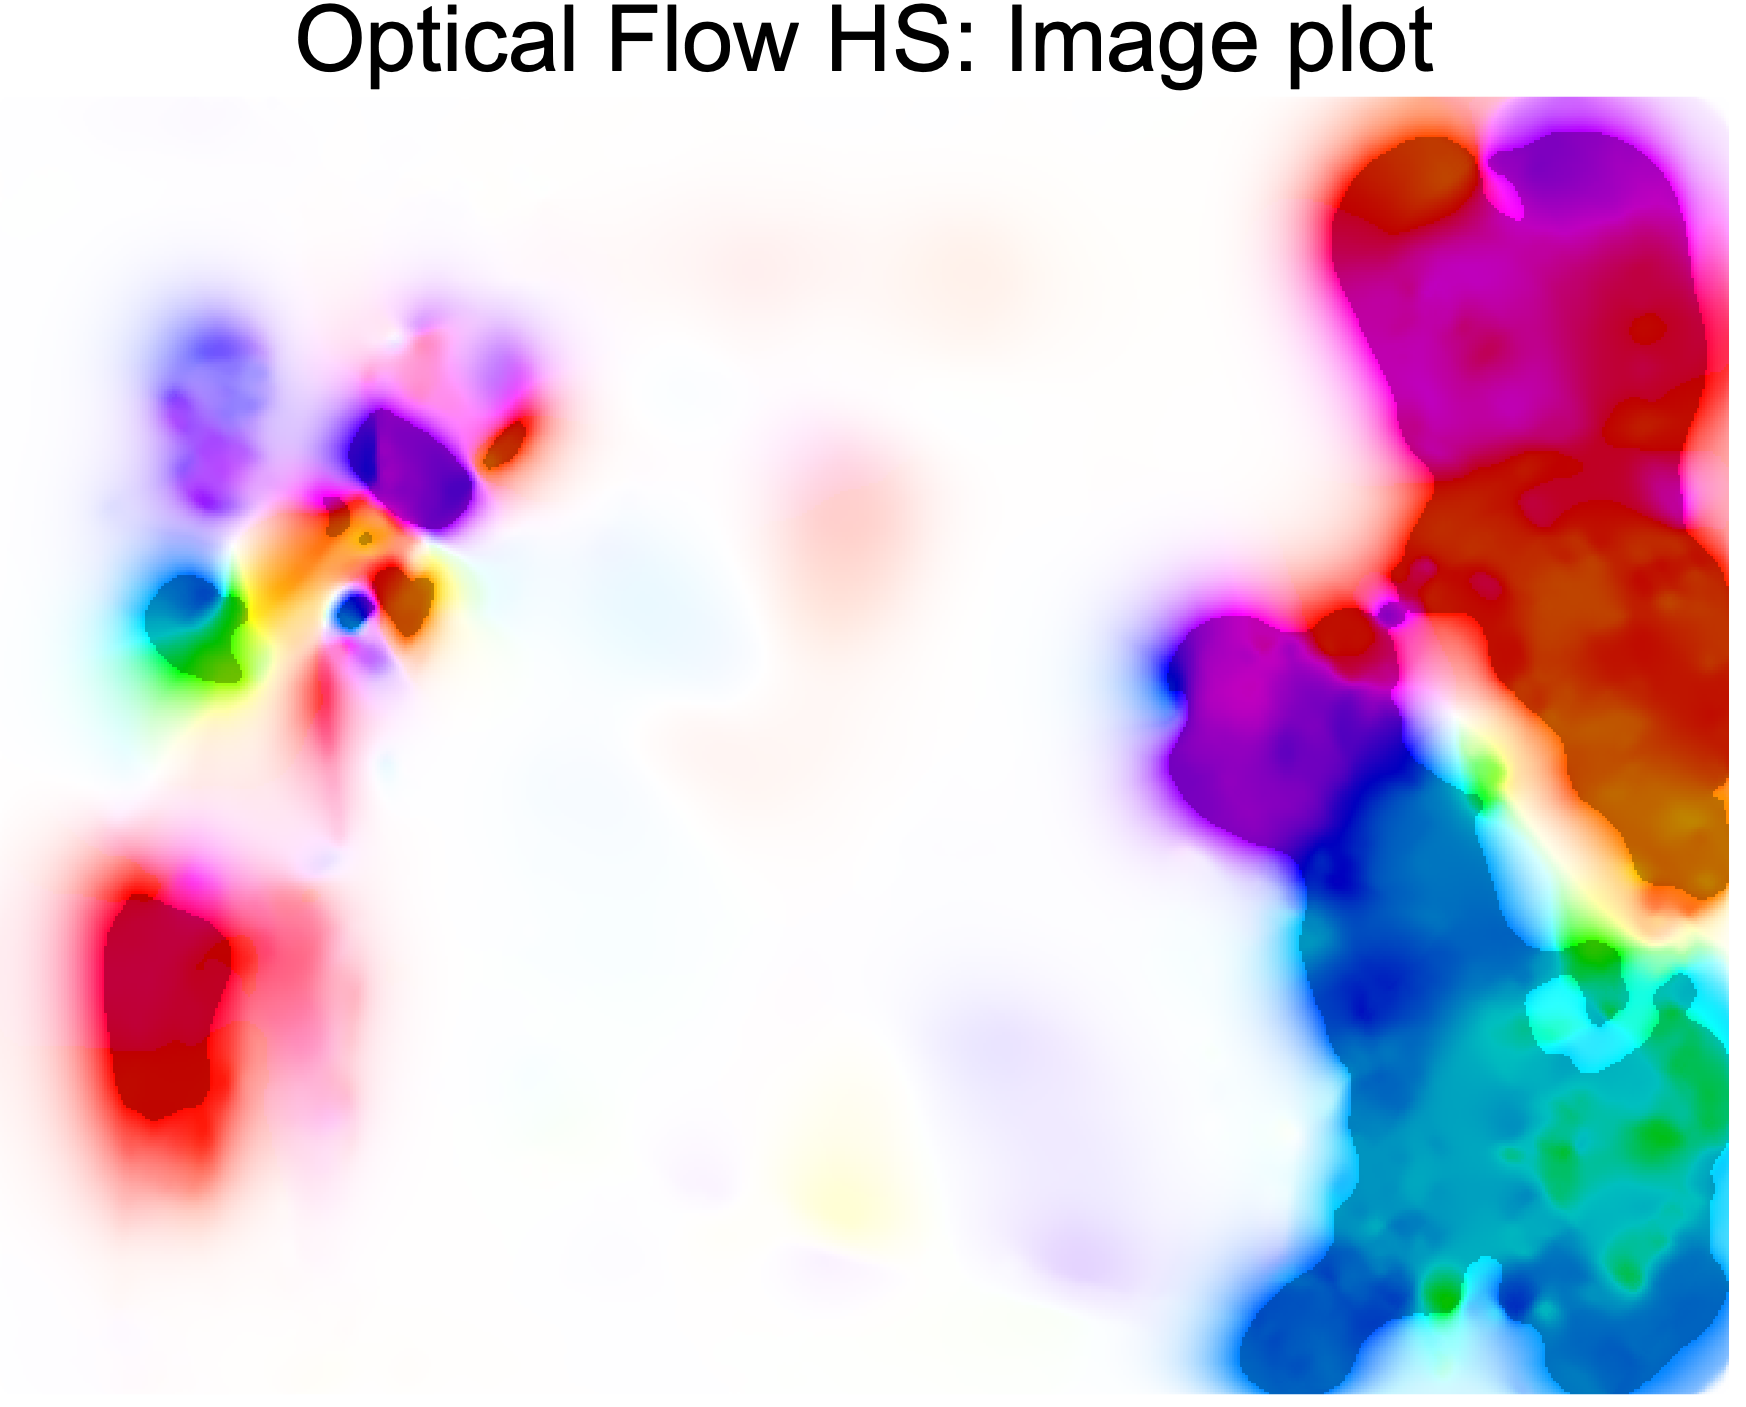
\includegraphics[width=0.16\linewidth]{figures/basketball/Basketball_HS_rgb.png}\\[-0.1em]
   \multicolumn{6}{c}{\smaller Evergreen} &\\[-0.2em]
   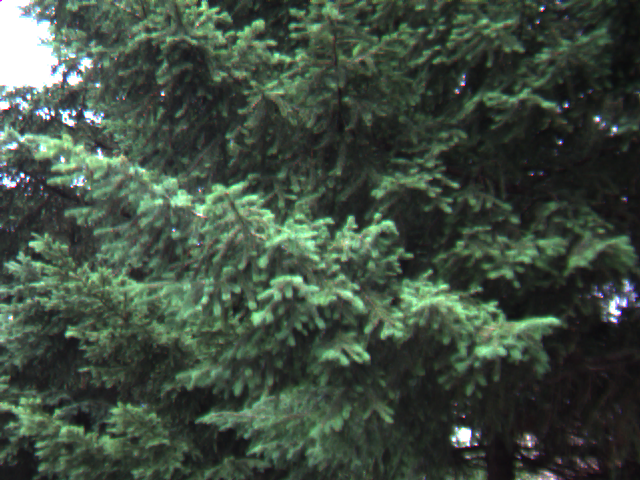
\includegraphics[width=0.16\linewidth]{figures/Evergreen/frame10.png}&
   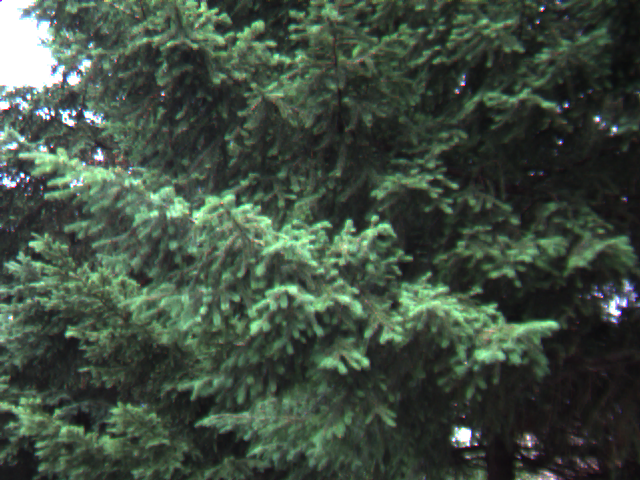
\includegraphics[width=0.16\linewidth]{figures/Evergreen/frame11.png}&
   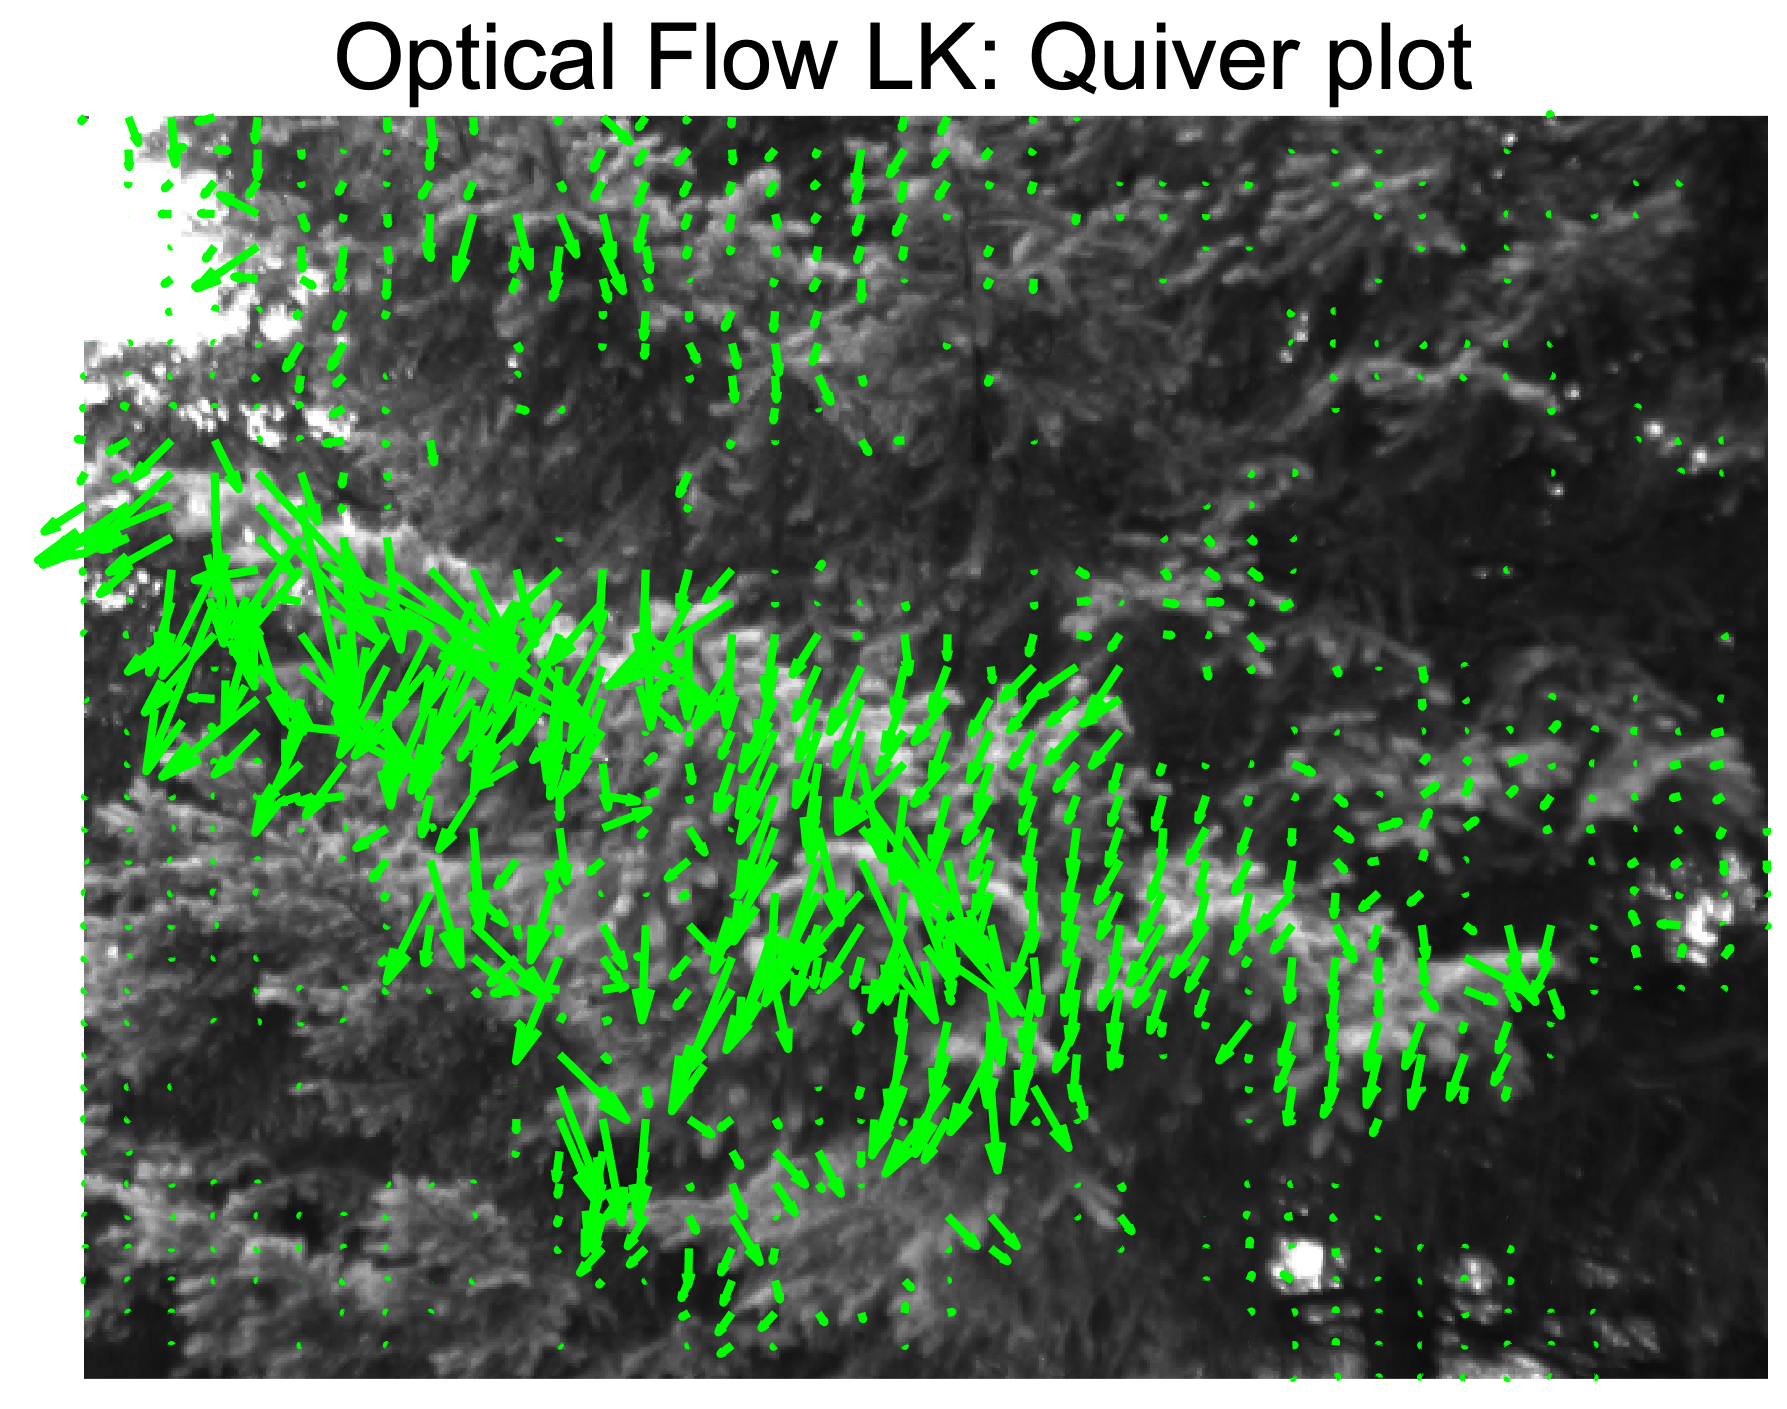
\includegraphics[width=0.16\linewidth]{figures/Evergreen/Evergreen_LK_quiver.png}&
   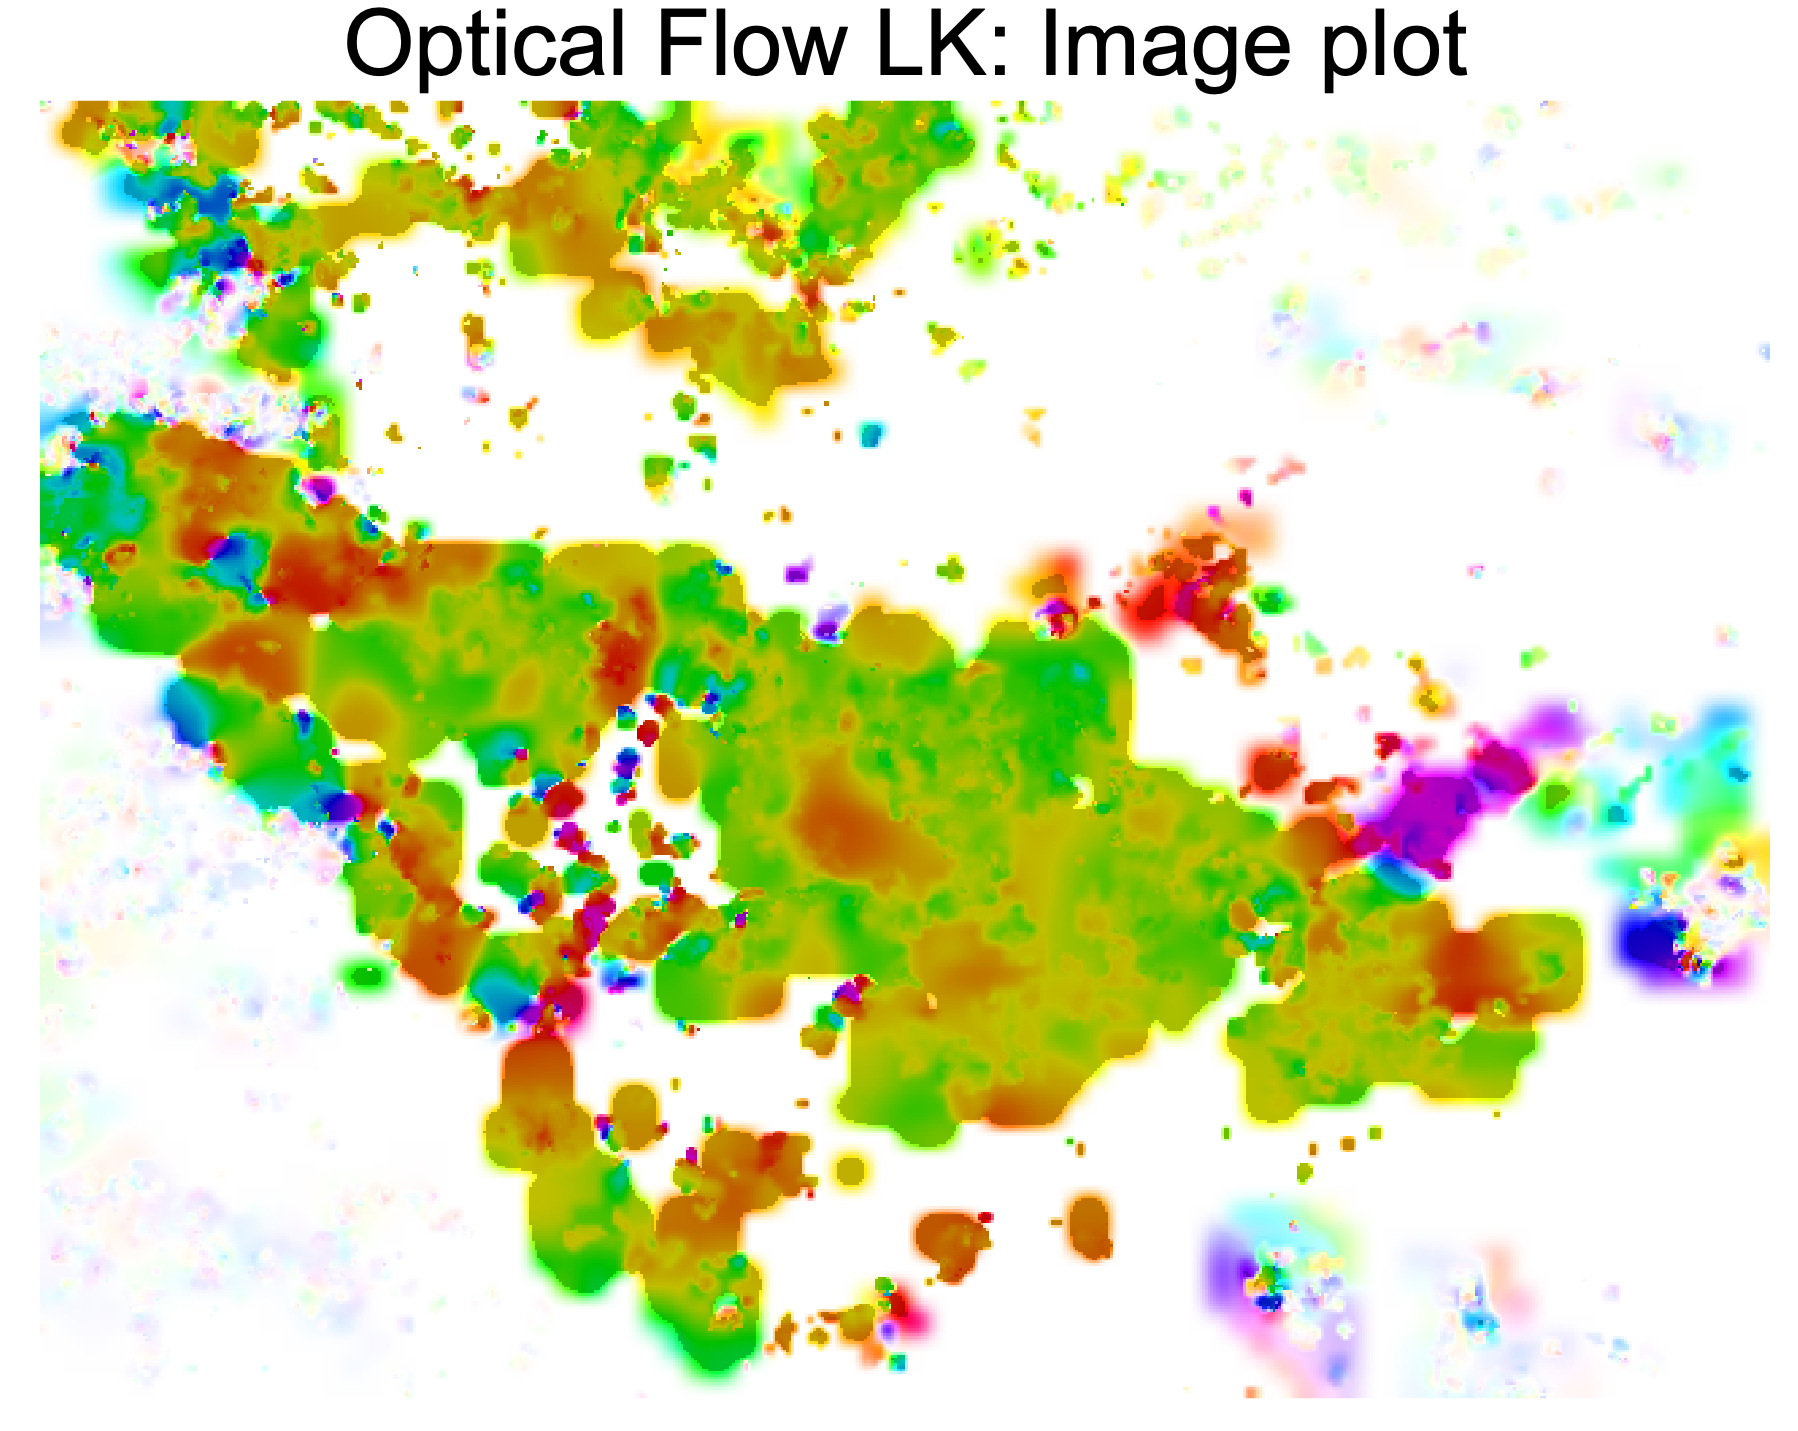
\includegraphics[width=0.16\linewidth]{figures/Evergreen/Evergreen_LK_rgb.png}&
   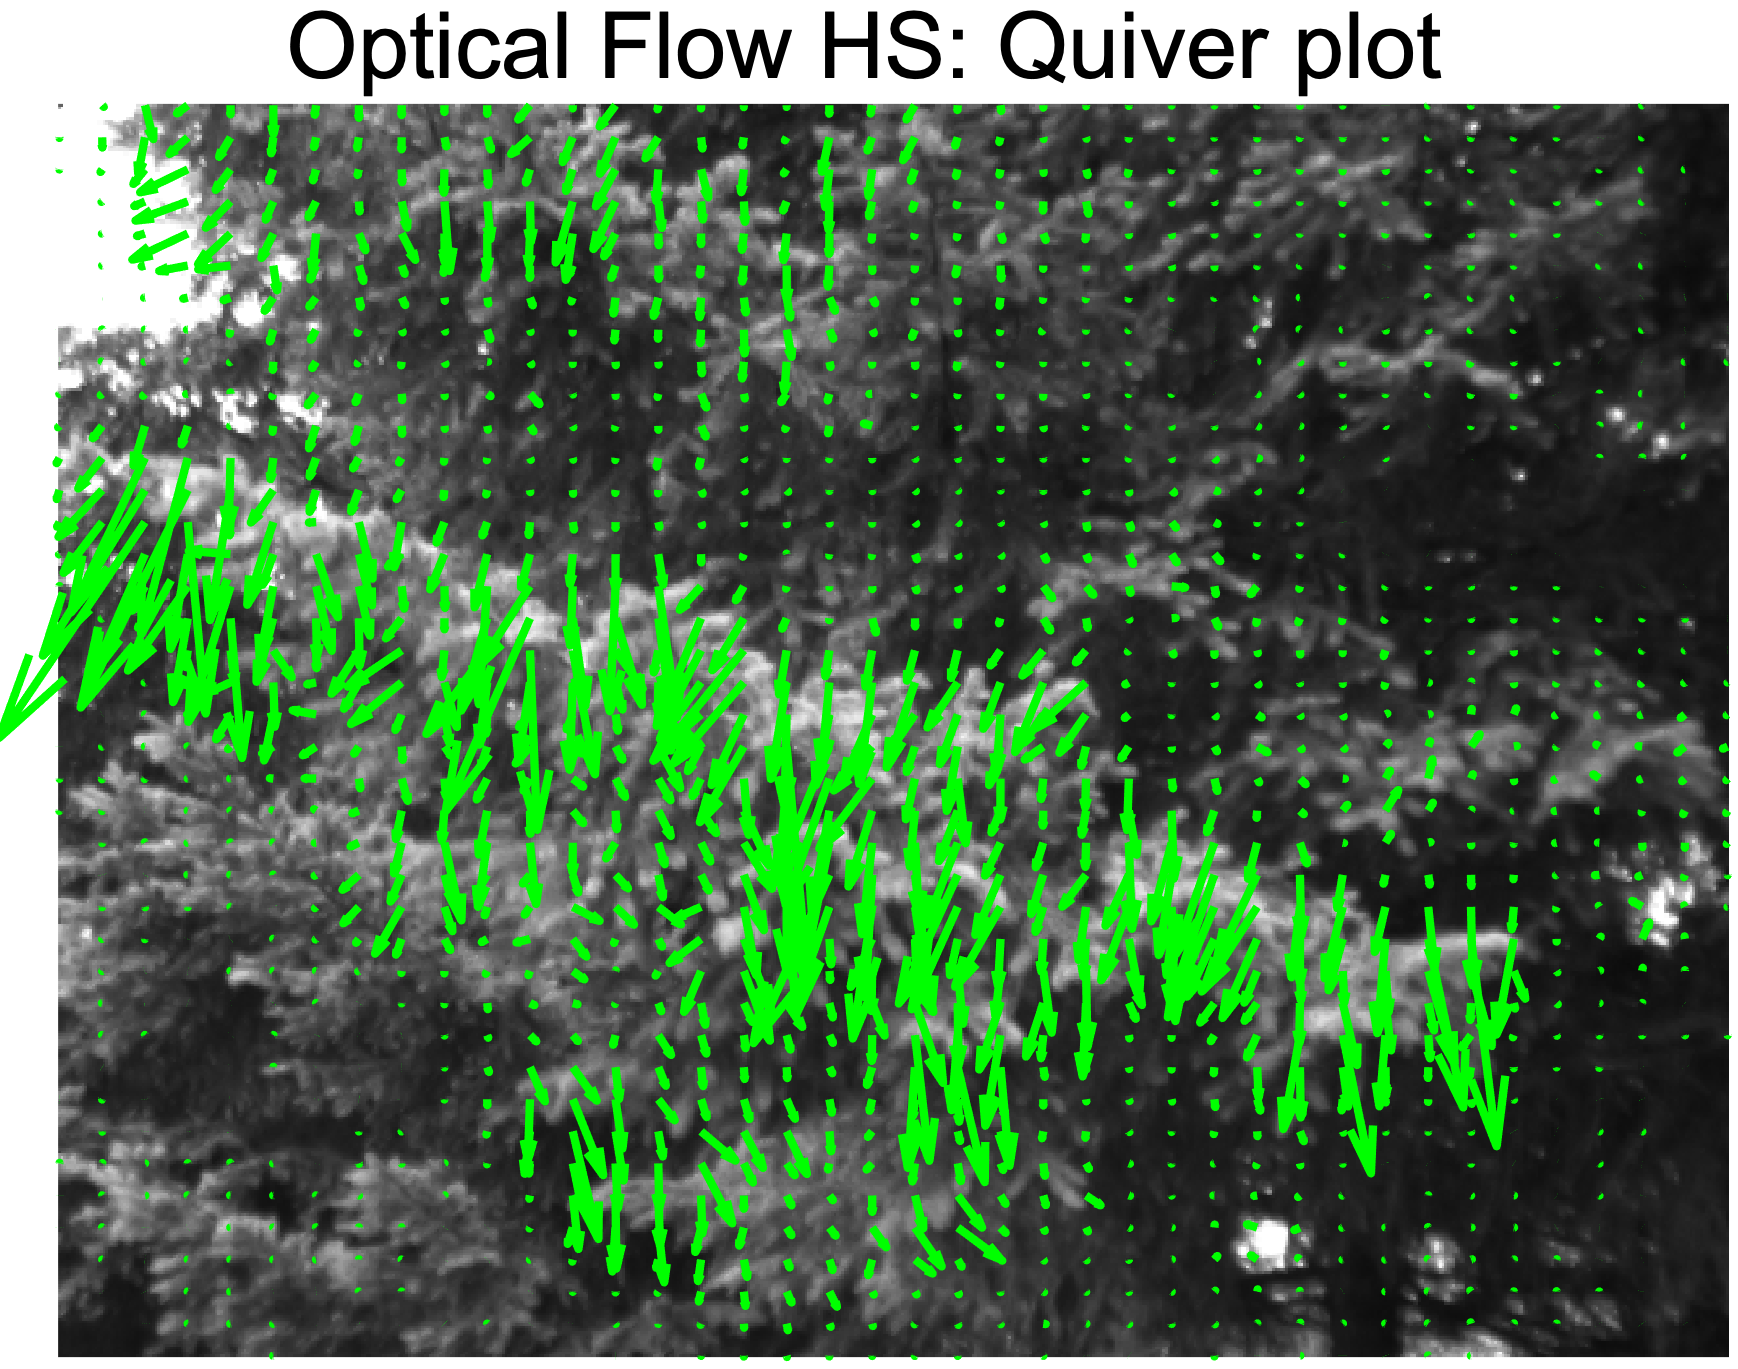
\includegraphics[width=0.16\linewidth]{figures/Evergreen/Evergreen_HS_quiver.png}&
   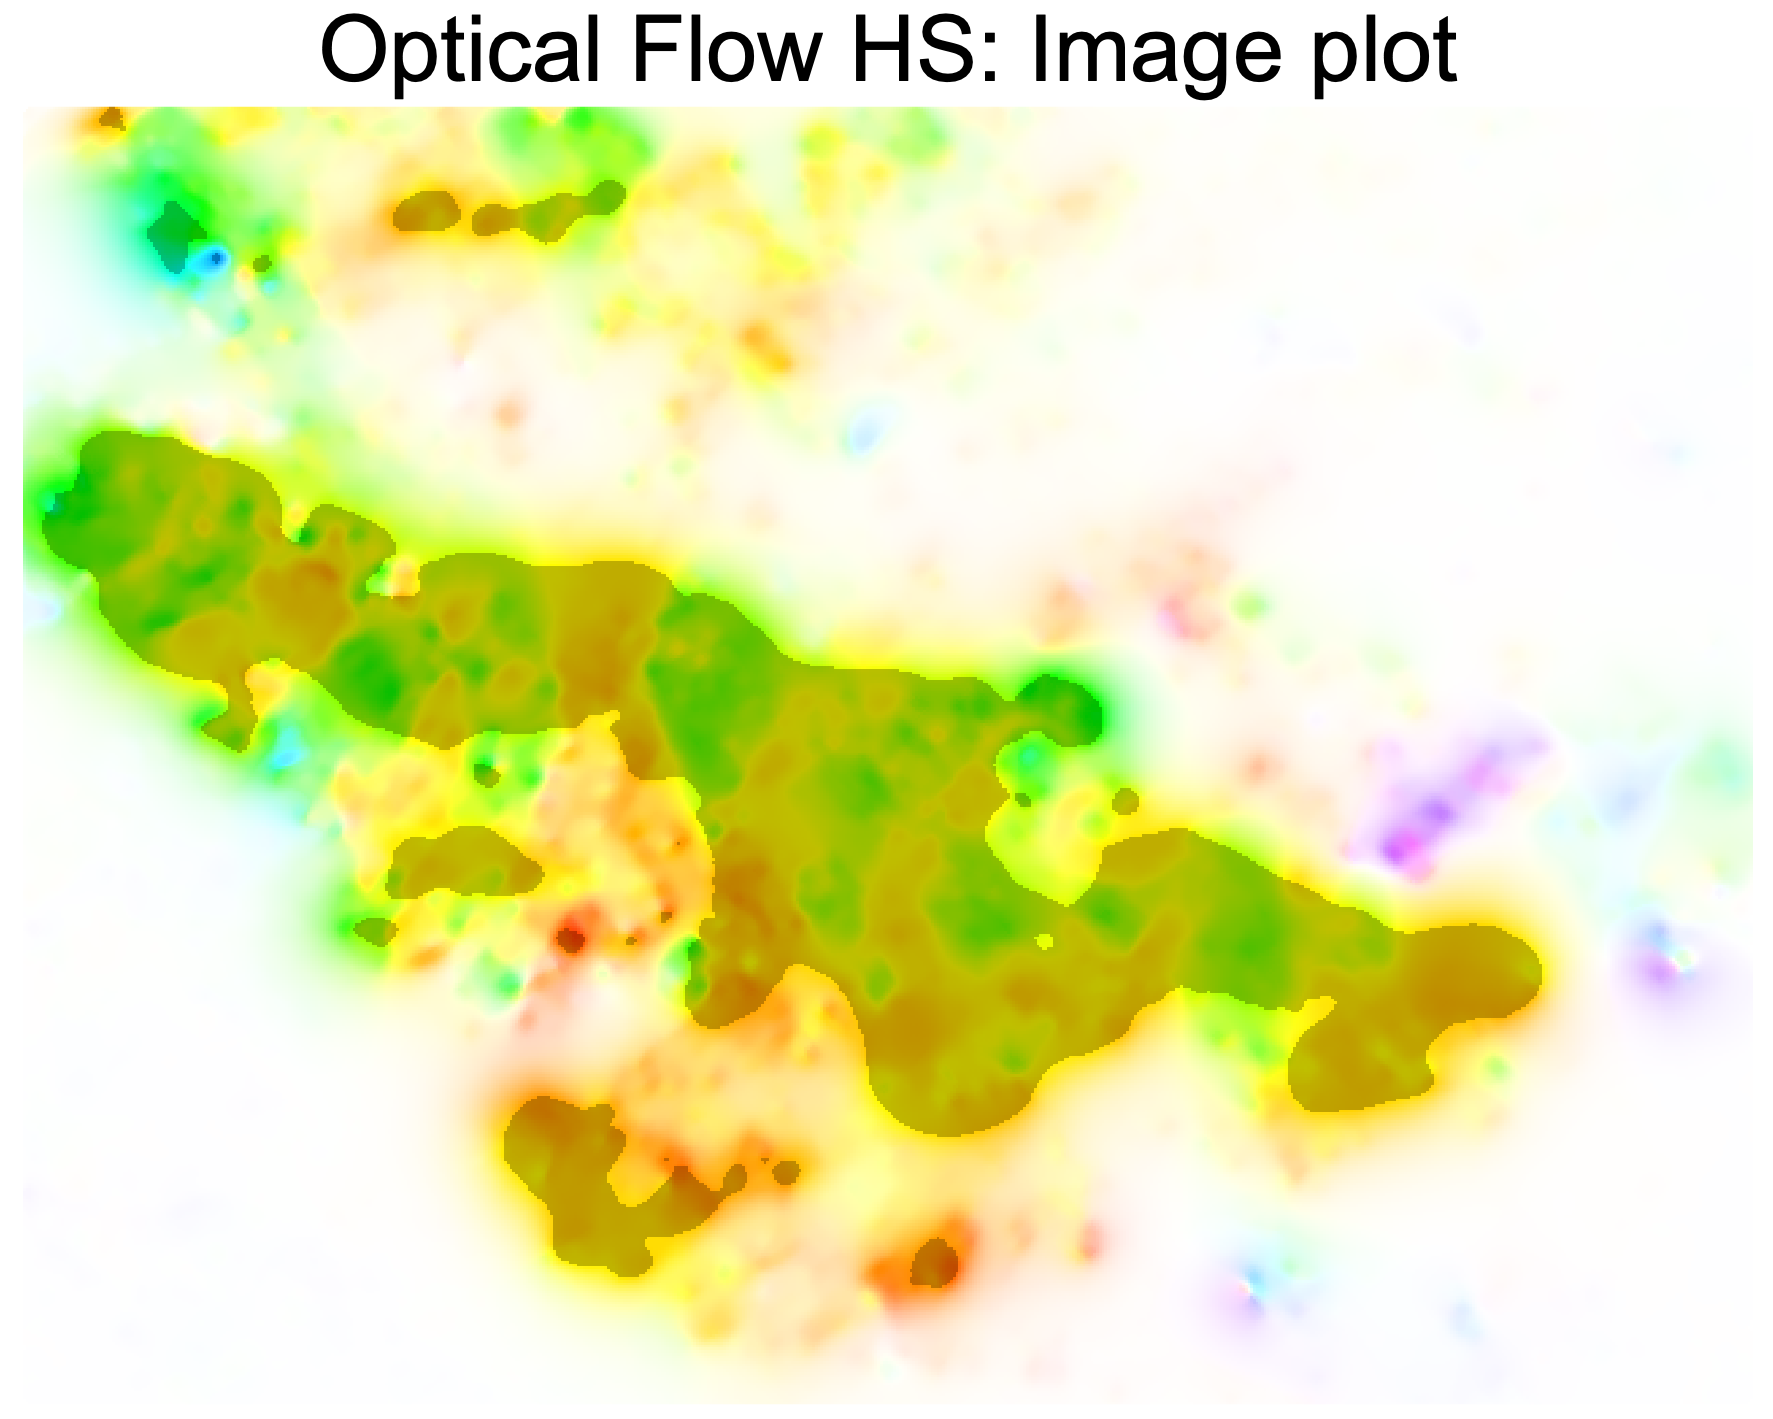
\includegraphics[width=0.16\linewidth]{figures/Evergreen/Evergreen_HS_rgb.png}\\[-0.1em]
   \multicolumn{6}{c}{\smaller Wooden} &\\[-0.2em]
	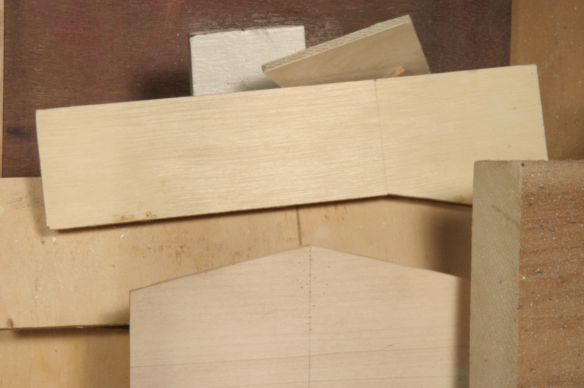
\includegraphics[width=0.16\linewidth]{figures/Wooden/frame10.png}&
	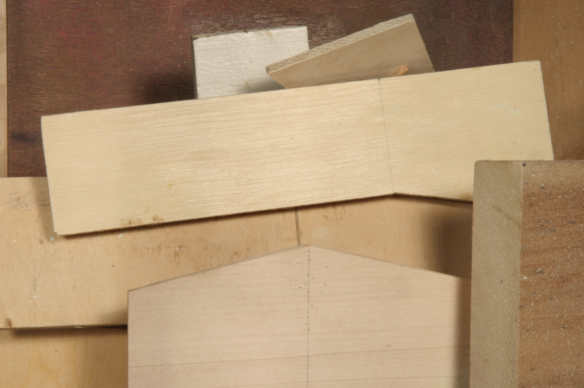
\includegraphics[width=0.16\linewidth]{figures/Wooden/frame11.png}&
	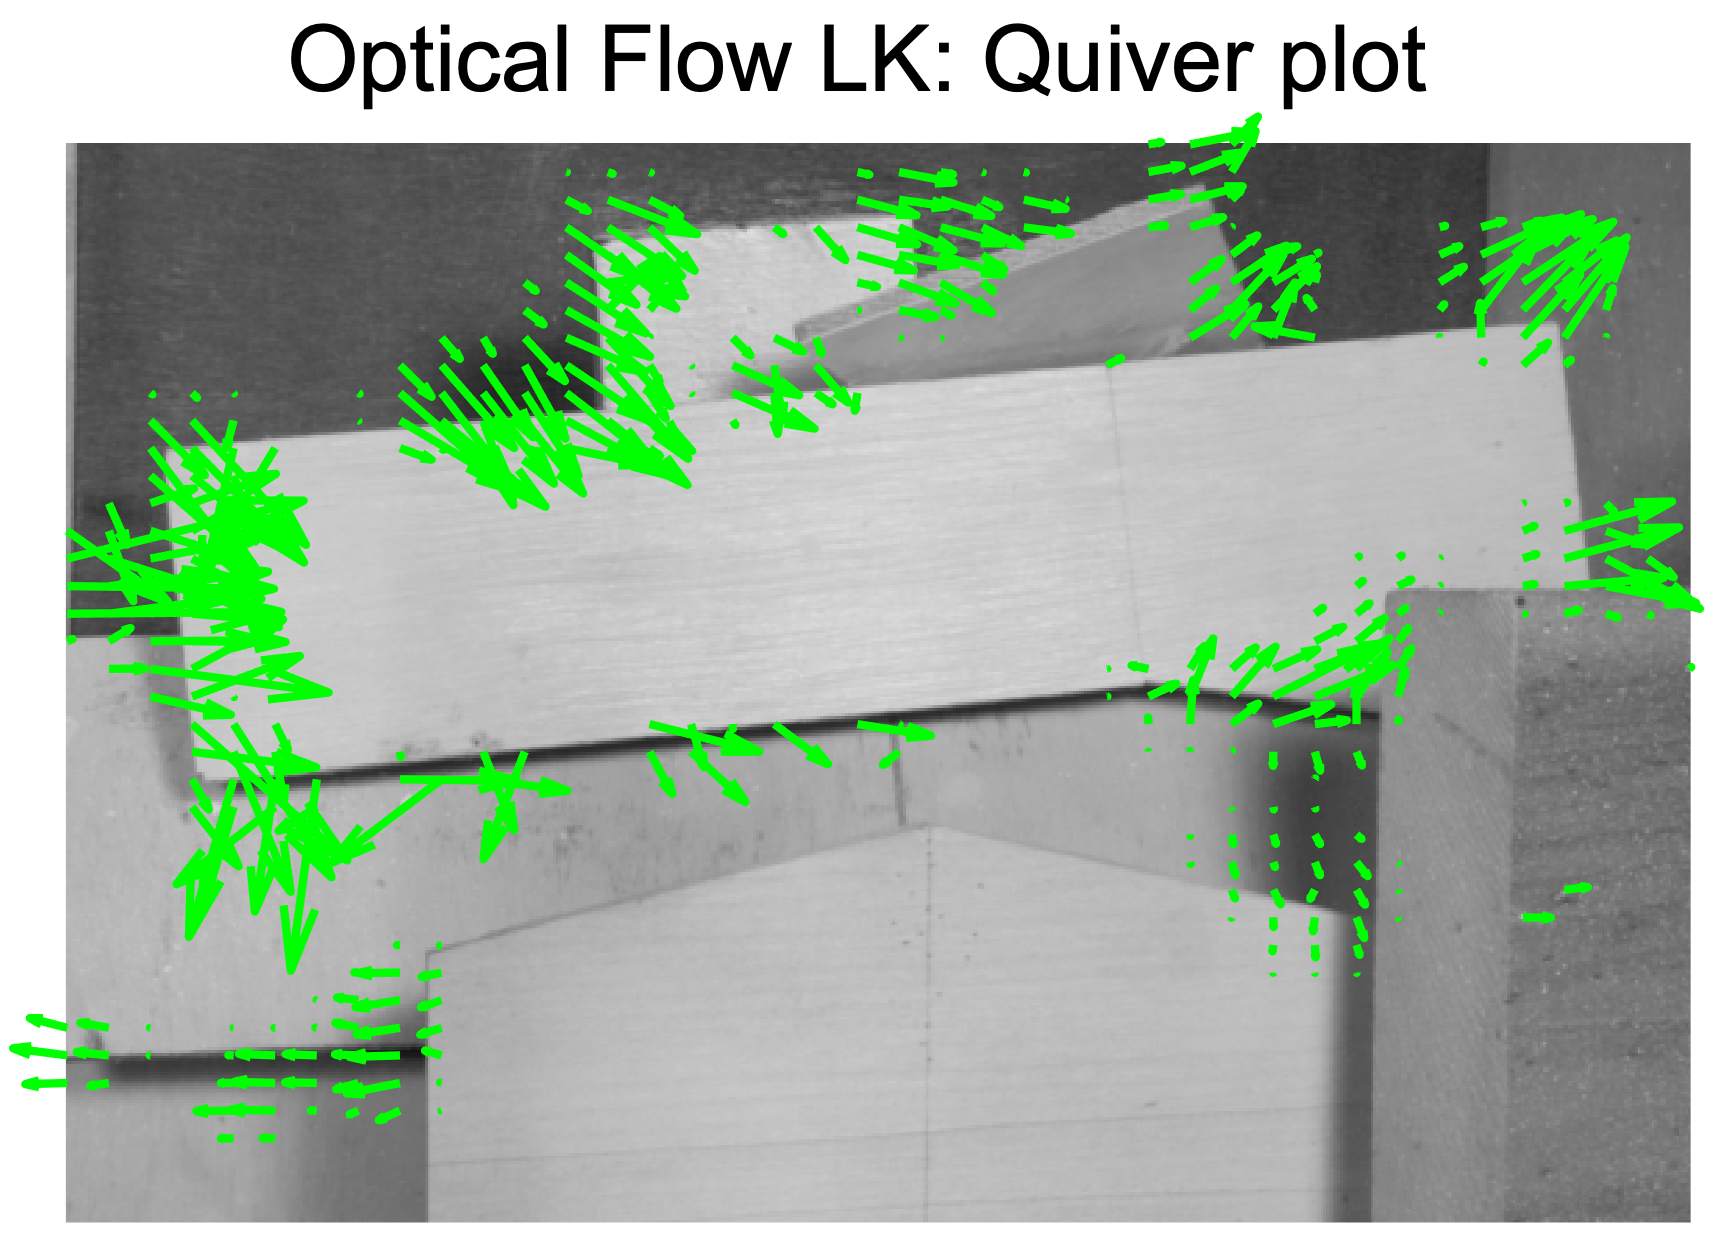
\includegraphics[width=0.16\linewidth]{figures/Wooden/Wooden_LK_quiver.png}&
	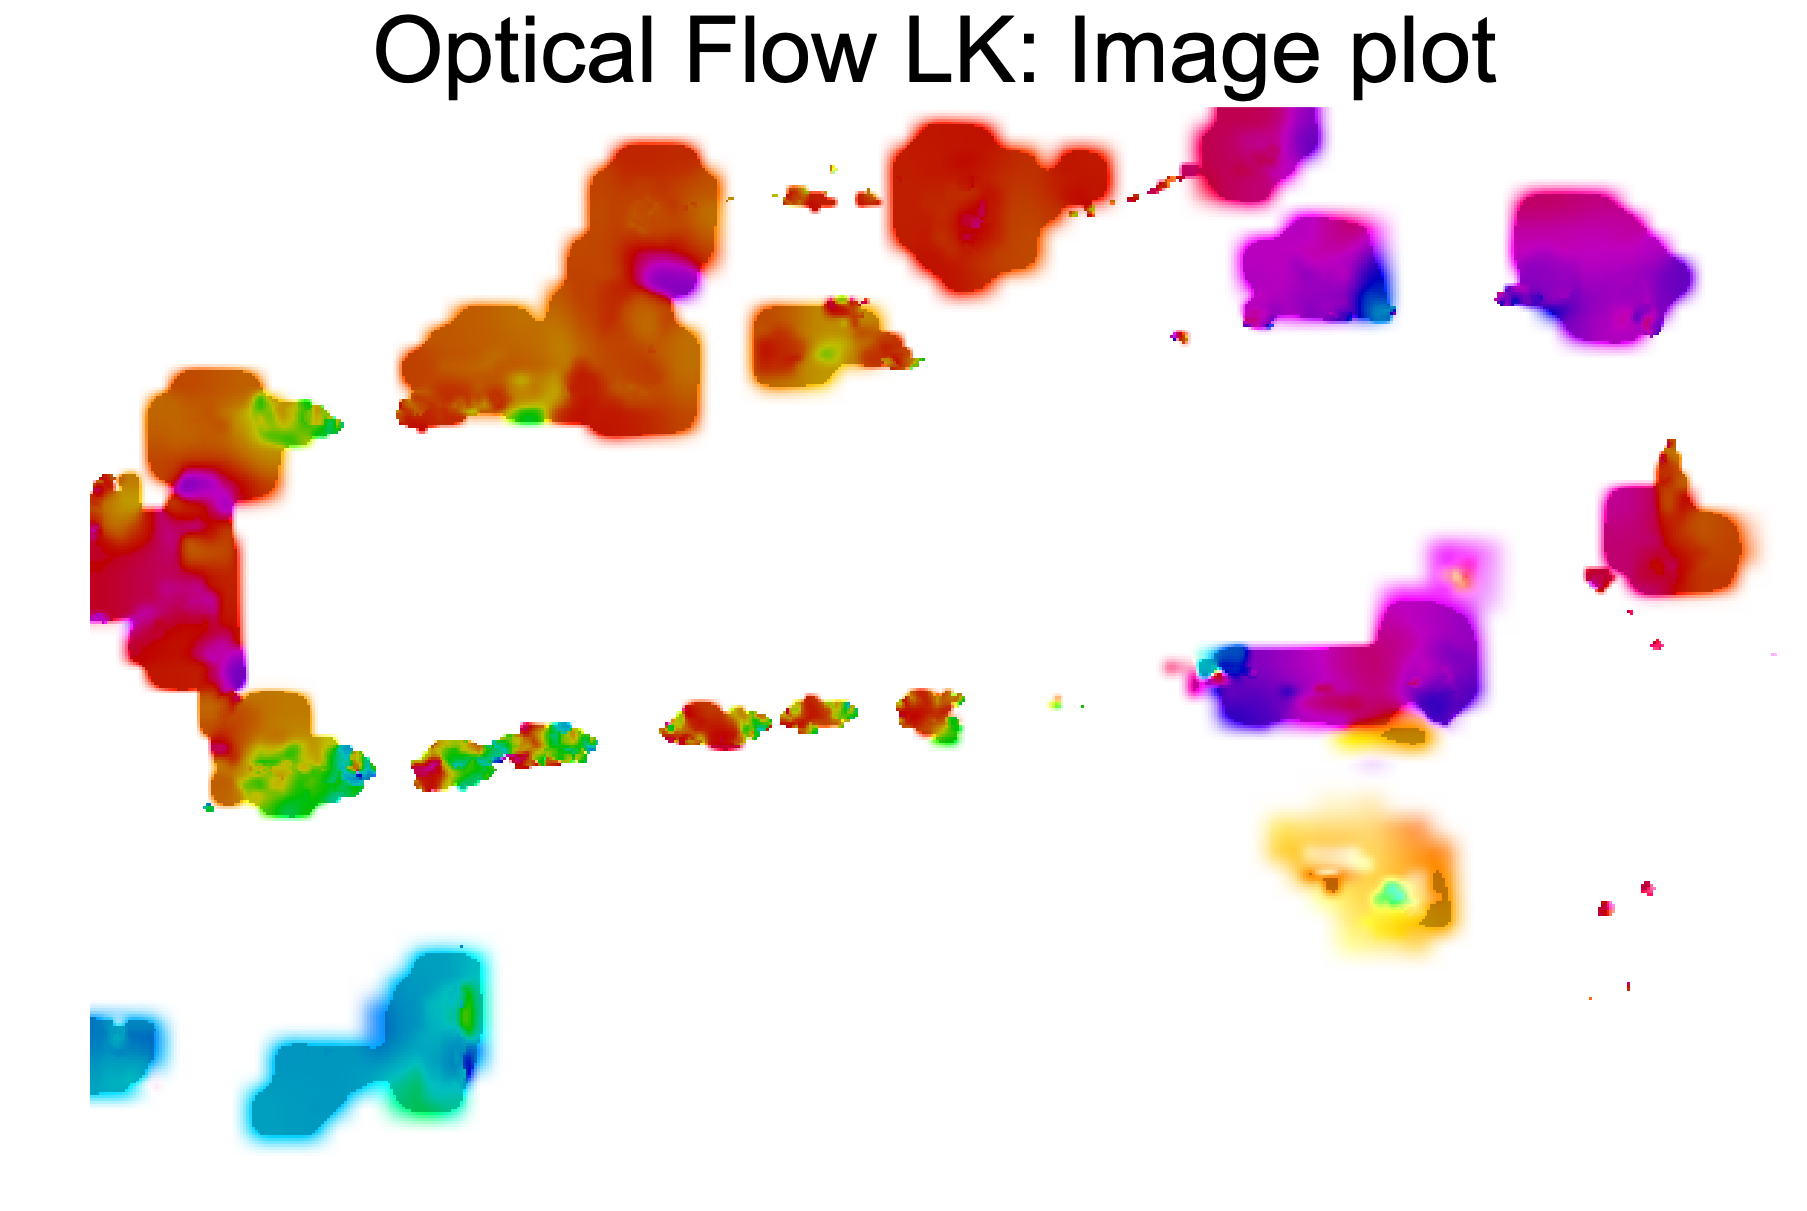
\includegraphics[width=0.16\linewidth]{figures/Wooden/Wooden_LK_rgb.png}&
	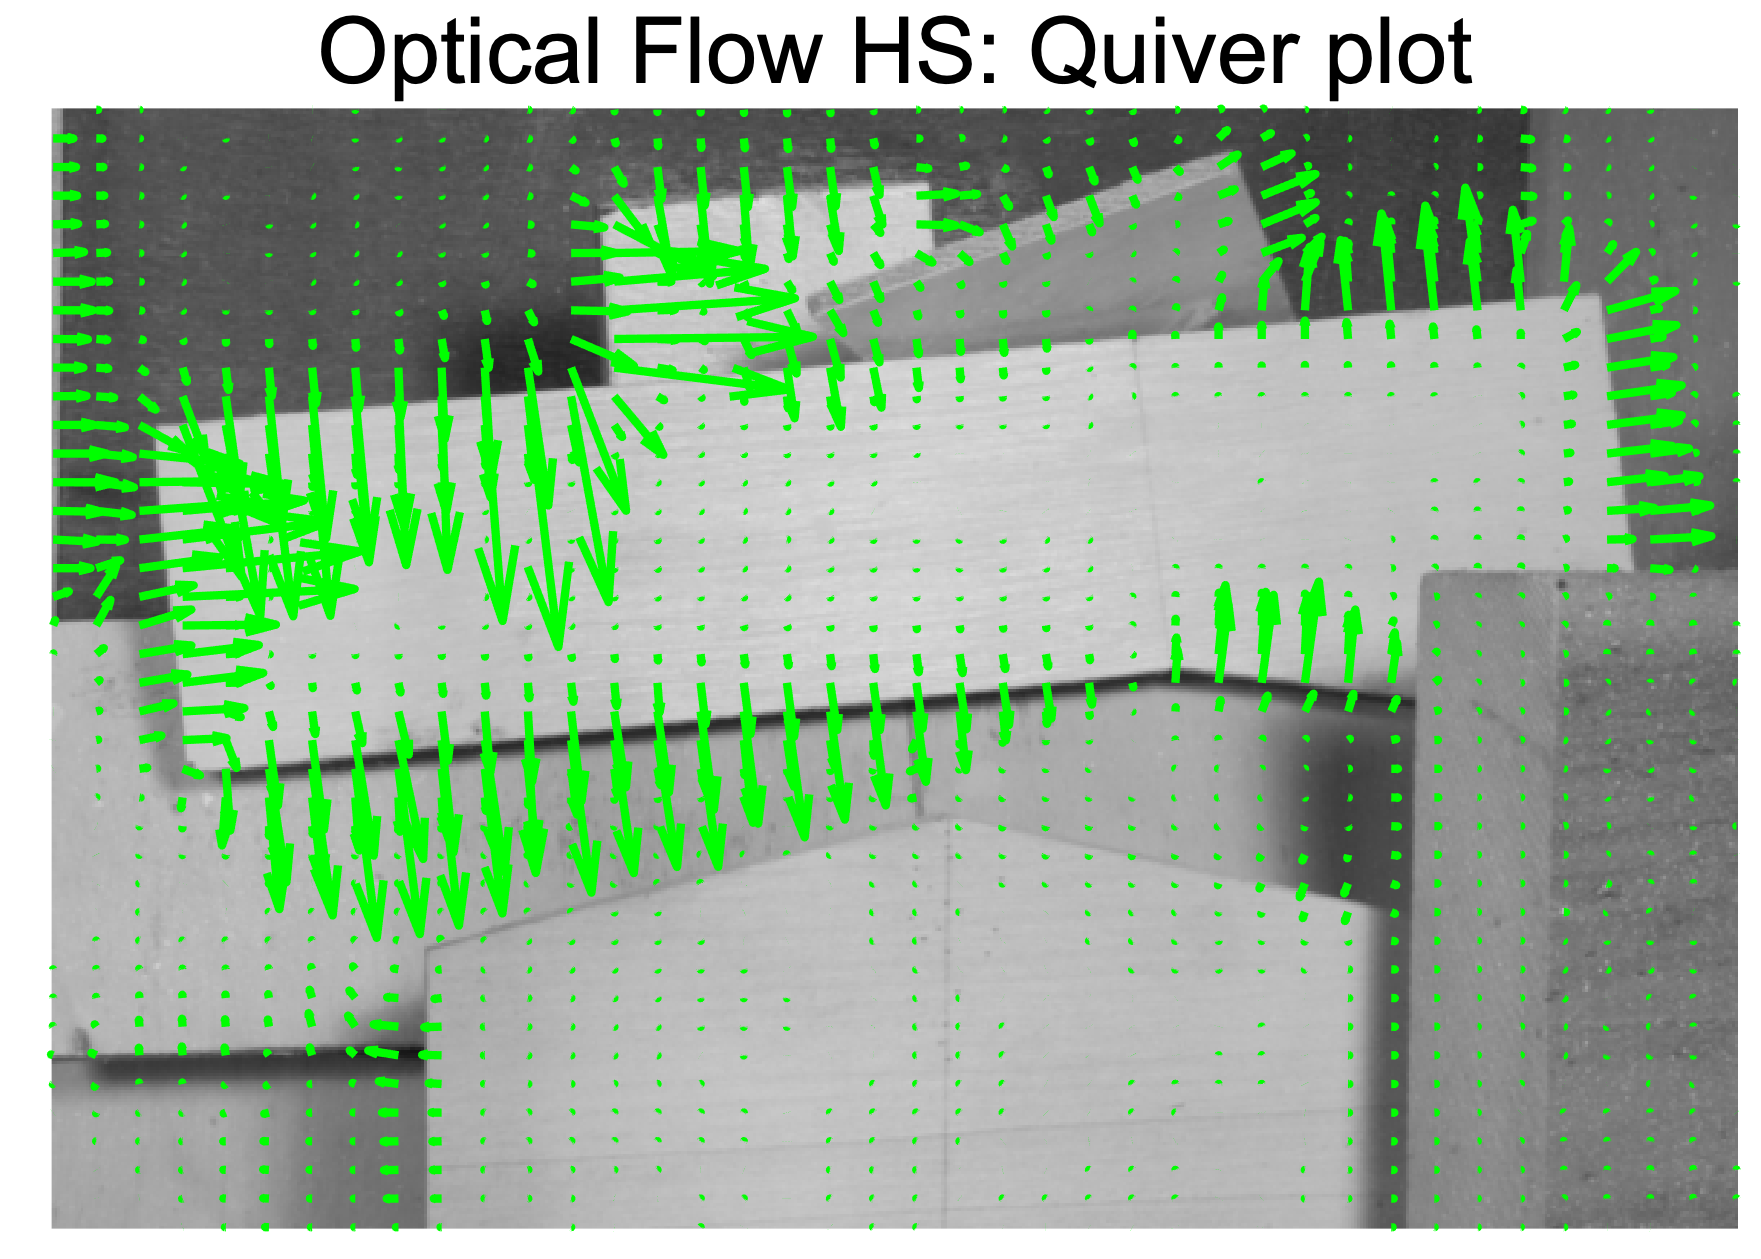
\includegraphics[width=0.16\linewidth]{figures/Wooden/Wooden_HS_quiver.png}&
	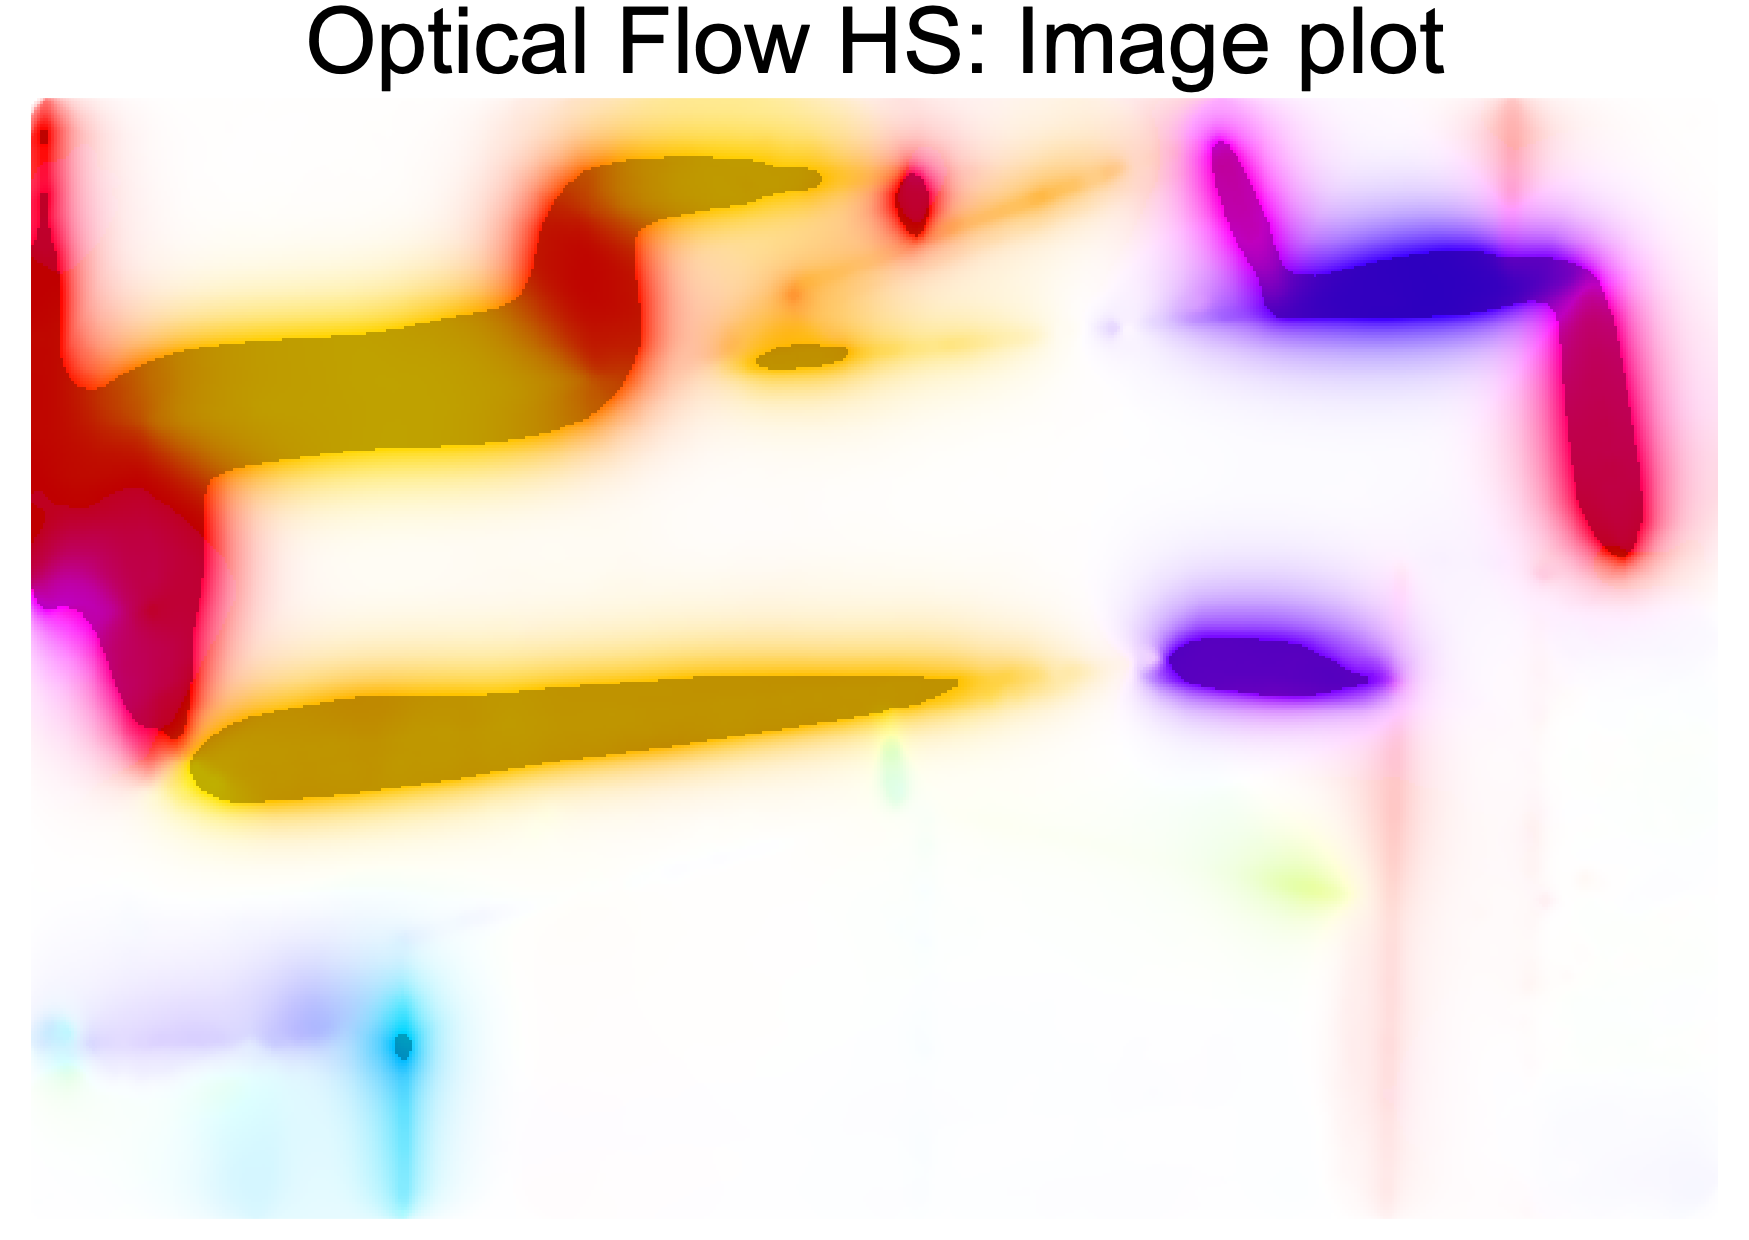
\includegraphics[width=0.16\linewidth]{figures/Wooden/Wooden_HS_rgb.png}\\[-0.1em]

   \smaller Image $1$ & \smaller Image $2$ & \smaller LK Quiver Plot & \smaller LK Flow Image & \smaller HS Quiver Plot & \smaller HS Flow Image
   \end{tabular}
   }
%
% %%%%%%%%%%%%%%%%%%%%%%%%%%%%%%%%%%%%%%%%%%%%%%%%%%%%%%%%%%%%%%%%%%%%%%%%%%%%%%
%   \headerbox{Methods Compared}{name=methods,column=0,below=algorithm}{
% %%%%%%%%%%%%%%%%%%%%%%%%%%%%%%%%%%%%%%%%%%%%%%%%%%%%%%%%%%%%%%%%%%%%%%%%%%%%%%
%   \begin{tabular}{rllllll}
%     Method                              & Hessian               &                                        & Gradient        &                                  & Speed      & Capture Range\\
%     \midrule
% \CoDe{} (this paper)                & Not used              &                                        & True:           & $\tilde{J}_{\qq_0}^T\e{\qq_0}$   & Fast       & Large  \\[0.1em]
% \LinCoDe{} (this paper)             & Not used              &                                        & Linear Approx:  & $\bar{J}^T\e{\qq_0}$             & Very Fast  & Medium \\[0.1em]
% \CoLiNe{}~\cite{burkhardt86:motion} & Constant Approx.:     & $\bar{J}^T\bar{J}$                     & True:           & $\tilde{J}_{\qq_0}^T\e{\qq_0}$   & Fast       & Medium \\[0.1em]
% \ICIA{}~\cite{matthews:aamr}        & Constant Approx.:     & $\bar{J}^T\bar{J}$                     & Linear Approx:  & $\bar{J}^T\e{\qq_0}$             & Very Fast  & Small  \\[0.1em]
% \CoNe{}~\cite{matthews:kanade20}    & Gauss-Newton Approx.: & $\tilde{J}_{\qq_0}^T\tilde{J}_{\qq_0}$ & True:           & $\tilde{J}_{\qq_0}^T\e{\qq_0}$   & Slow       & Large  
%   \end{tabular}
%   The methods introduced in this paper are Hessian-free gradient descent methods.
%  }
%
 %%%%%%%%%%%%%%%%%%%%%%%%%%%%%%%%%%%%%%%%%%%%%%%%%%%%%%%%%%%%%%%%%%%%%%%%%%%%%%
   \headerbox{References}{name=references,column=1,above=bottom}{
 %%%%%%%%%%%%%%%%%%%%%%%%%%%%%%%%%%%%%%%%%%%%%%%%%%%%%%%%%%%%%%%%%%%%%%%%%%%%%%
     \smaller
     
     \bibliographystyle{ieee}
     \renewcommand{\section}[2]{\vskip 0.05em}
       \begin{thebibliography}{99}\itemsep=-0.01em
       \setlength{\baselineskip}{0.4em}
       \bibitem{flow:lucas} Lucas~B~D,~Kanade~T.
 	    An iterative image registration technique with an application to stereo vision[J]. 1981.     
 	   \bibitem{flow:horns} 
 	   Horn B K P, Schunck B G. 
 	   \newblock Determining optical flow[J].
 	   \newblock  Artificial intelligence, 1981. 
       \end{thebibliography}
   }

 %%%%%%%%%%%%%%%%%%%%%%%%%%%%%%%%%%%%%%%%%%%%%%%%%%%%%%%%%%%%%%%%%%%%%%%%%%%%%%
%   \headerbox{Training + Testing Data}{name=data,column=0,above=references,below=abstract}{
% %%%%%%%%%%%%%%%%%%%%%%%%%%%%%%%%%%%%%%%%%%%%%%%%%%%%%%%%%%%%%%%%%%%%%%%%%%%%%%
%   \includegraphics[width=0.2\linewidth]{018_4_2_masked}%
%   \includegraphics[width=0.2\linewidth]{328_2_1_masked}%
%   \includegraphics[width=0.2\linewidth]{319_2_1_masked}%
%   \includegraphics[width=0.2\linewidth]{027_4_2_masked}%
%   \includegraphics[width=0.2\linewidth]{020_1_1_masked}
%   \includegraphics[width=0.2\linewidth]{12_2f_masked}%
%   \includegraphics[width=0.2\linewidth]{21_3m_masked}%
%   \includegraphics[width=0.2\linewidth]{09_6m_masked}%
%   \includegraphics[width=0.2\linewidth]{33_4m_masked}%
%   %\includegraphics[width=0.2\linewidth]{22_3f_masked}
%   $\dots$\\
%   The model was trained from 456 images from the IMM and XM2VTS datasets using
%   120 landmarks. Get the landmarks, model, and source code at:\\
%   \mbox{\url{www.cs.unibas.ch/personen/amberg_brian/aam/}}
%   }

 %%%%%%%%%%%%%%%%%%%%%%%%%%%%%%%%%%%%%%%%%%%%%%%%%%%%%%%%%%%%%%%%%%%%%%%%%%%%%%

   \headerbox{Tracking 5000 frames with a general model}{name=tracking,column=2,span=2,below=speed,above=bottom}{
 %%%%%%%%%%%%%%%%%%%%%%%%%%%%%%%%%%%%%%%%%%%%%%%%%%%%%%%%%%%%%%%%%%%%%%%%%%%%%%
% \begin{tabular}{c@{\hspace{0.05em}}c@{\hspace{0.1em}}c@{\hspace{0.1em}}c@{\hspace{0.1em}}c@{\hspace{1em}}c@{\hspace{0.1em}}c@{\hspace{0.1em}}c@{\hspace{0.1em}}c@{\hspace{0.1em}}c}
%   \multicolumn{5}{c}{\smaller \ICIA{} with $\VLins$} &
%   \multicolumn{5}{c}{\smaller \ICIA{} with $\VLins$ + Regularisation}\\[-0.2em]
%   \includegraphics[width=0.095\linewidth]{track_frame_00010_01}&
%   \includegraphics[width=0.095\linewidth]{track_frame_00050_01}&
%   \includegraphics[width=0.095\linewidth]{track_frame_00450_01}&
%   \includegraphics[width=0.095\linewidth]{track_frame_02000_01}&
%   \includegraphics[width=0.095\linewidth]{track_frame_04999_01}&
%   %
%   \includegraphics[width=0.095\linewidth]{track_frame_00010_02}&
%   \includegraphics[width=0.095\linewidth]{track_frame_00050_02}&
%   \includegraphics[width=0.095\linewidth]{track_frame_00450_02}&
%   \includegraphics[width=0.095\linewidth]{track_frame_02000_02}&
%   \includegraphics[width=0.095\linewidth]{track_frame_04999_02}\\[-0.1em]
%   %
%   \multicolumn{5}{c}{\smaller \LinCoDe{}} &
%   \multicolumn{5}{c}{\smaller \LinCoDe{} + Regularisation}\\[-0.2em]
%   \includegraphics[width=0.095\linewidth]{track_frame_00010_03}&
%   \includegraphics[width=0.095\linewidth]{track_frame_00050_03}&
%   \includegraphics[width=0.095\linewidth]{track_frame_00450_03}&
%   \includegraphics[width=0.095\linewidth]{track_frame_02000_03}&
%   \includegraphics[width=0.095\linewidth]{track_frame_04999_03}&
%   %
%   \includegraphics[width=0.095\linewidth]{track_frame_00010_04}&
%   \includegraphics[width=0.095\linewidth]{track_frame_00050_04}&
%   \includegraphics[width=0.095\linewidth]{track_frame_00450_04}&
%   \includegraphics[width=0.095\linewidth]{track_frame_02000_04}&
%   \includegraphics[width=0.095\linewidth]{track_frame_04999_04}\\[-0.1em]
%   %
%   \multicolumn{5}{c}{\smaller \CoDe{}} &
%   \multicolumn{5}{c}{\smaller \CoDe{} + Regularisation}\\[-0.2em]
%   \includegraphics[width=0.095\linewidth]{track_frame_00010_05}&
%   \includegraphics[width=0.095\linewidth]{track_frame_00050_05}&
%   \includegraphics[width=0.095\linewidth]{track_frame_00450_05}&
%   \includegraphics[width=0.095\linewidth]{track_frame_02000_05}&
%   \includegraphics[width=0.095\linewidth]{track_frame_04999_05}&
%   %
%   \includegraphics[width=0.095\linewidth]{track_frame_00010_06}&
%   \includegraphics[width=0.095\linewidth]{track_frame_00050_06}&
%   \includegraphics[width=0.095\linewidth]{track_frame_00450_06}&
%   \includegraphics[width=0.095\linewidth]{track_frame_02000_06}&
%   \includegraphics[width=0.095\linewidth]{track_frame_04999_06}\\[-0.5em]
%   \smaller Frame 10 & \smaller Frame 50 & \smaller Frame 450 & \smaller Frame 2000 & \smaller Frame 5000 &
%   \smaller Frame 10 & \smaller Frame 50 & \smaller Frame 450 & \smaller Frame 2000 & \smaller Frame 5000
%   \end{tabular}
% }
%   \vspace{-1.2em}
%   \begin{multicols}{2}
%   {\textbf{Our algorithm makes fast and robust tracking possible.}
%     We compare face tracking under natural motion, using \ICIA{},
%     \LinCoDe{} and \CoDe{}. The original \ICIA{} fails
%     immediately with this large model and new face data. Substituting the orthonormal
%     incremental warp for the original \ICIA{} warp, the algorithm still loses track
%     very early, whereas \LinCoDe{} and \CoDe{} can track much
%     further. Finally, adding regularisation to all algorithms, \ICIA{} still
%     loses track completely after approximately 500 frames and does not recover
%     the local deformations accurately. In contrast \CoDe{} now tracks the full
%     5000 frame sequence without reinitialization, and \LinCoDe{} tracks for 2500 frames.}
%   
%   The same training dataset was used for both tracking experiments. The
%   training data was aquired with different camera and light settings from
%   different subjects.
%   \end{multicols}
   }
 %%%%%%%%%%%%%%%%%%%%%%%%%%%%%%%%%%%%%%%%%%%%%%%%%%%%%%%%%%%%%%%%%%%%%%%%%%%%%%
%   \headerbox{Low Res Tracking}{name=lowrestracking,column=1,span=1,below=speed,above=bottom}{
 %%%%%%%%%%%%%%%%%%%%%%%%%%%%%%%%%%%%%%%%%%%%%%%%%%%%%%%%%%%%%%%%%%%%%%%%%%%%%%
%\begin{tabular}{@{}c@{}c@{}c@{}c@{}c@{}}
%  \multicolumn{5}{c}{\smaller \ICIA{} with $\VLins$}\\[-0.2em]
%  \includegraphics[width=0.2\linewidth]{bush_00010_02}&
%  \includegraphics[width=0.2\linewidth]{bush_00100_02}&
%  \includegraphics[width=0.2\linewidth]{bush_00200_02}&
%  \includegraphics[width=0.2\linewidth]{bush_00300_02}&
%  \includegraphics[width=0.2\linewidth]{bush_00400_02}\\[-0.1em]
%  \multicolumn{5}{c}{\smaller \LinCoDe{}}\\[-0.2em]
%  \includegraphics[width=0.2\linewidth]{bush_00010_05}&
%  \includegraphics[width=0.2\linewidth]{bush_00100_05}&
%  \includegraphics[width=0.2\linewidth]{bush_00200_05}&
%  \includegraphics[width=0.2\linewidth]{bush_00300_05}&
%  \includegraphics[width=0.2\linewidth]{bush_00400_05}\\[-0.1em]
%  \multicolumn{5}{c}{\smaller \CoDe{}}\\[-0.2em]
%  \includegraphics[width=0.2\linewidth]{bush_00010_08}&
%  \includegraphics[width=0.2\linewidth]{bush_00100_08}&
%  \includegraphics[width=0.2\linewidth]{bush_00200_08}&
%  \includegraphics[width=0.2\linewidth]{bush_00300_08}&
%  \includegraphics[width=0.2\linewidth]{bush_00400_08}\\[-0.5em]
%  \smaller Frame 10 & \smaller Frame 100 & \smaller Frame 200 & \smaller Frame 300 & \smaller Frame 400 
%  \end{tabular}

%  \vspace{1.25em}
%  \textbf{Tracking a low resolution video with large head motions
%  succeeds with \CoDe{}, where \ICIA{} fails.}\\ All methods used the orthonormal
%  incremental warp, and relatively strong regularisation.  \ICIA{} starts to
%  drift in the early frames, while~\CoDe{} tracks the full sequence. The
%  approximate gradient method \LinCoDe{} also suceeds, but looses
%  track of the details for about 100 frames.
%   }
 %%%%%%%%%%%%%%%%%%%%%%%%%%%%%%%%%%%%%%%%%%%%%%%%%%%%%%%%%%%%%%%%%%%%%%%%%%%%%%%
\end{poster}%
%
\end{document}
